\documentclass[12pt,a4paper,twoside]{book}
\usepackage[english]{babel}
\usepackage{graphicx}
\usepackage[font=small,labelfont=bf]{caption}
\usepackage{subcaption}
\usepackage{amsmath}

\newcommand{\norm}[1]{\lVert#1\rVert}

\bibliographystyle{abbrv}
\begin{document}

\begin{titlepage}
  \begin{center}
    \begin{Large}Universit\`a degli Studi di Trento\\\end{Large}
     Facolt\`a di Scienze Matematiche, Fisiche e Naturali\\
     \vspace{10pt}
     \begin{figure}[htbp]
       \begin{center}
         
\includegraphics[width=3cm]{images/sigillo_unitn.eps}
       \end{center}
     \end{figure}
Corso di Laurea in Informatica\\

\vspace{10pt}
\line(1,0){338}
\vspace{10pt}

Final Thesis\\
\end{center}
\vspace{3cm}
\begin{center}
\begin{Large}An Open Source implementation of a particle-based model for skiing dynamics\\\end{Large}
\vspace{3cm}
\end{center}
Relatore interno: \\ \textbf{Prof. Alberto Montresor} \\
Relatore esterno:\hspace{6.8cm}Laureando:   \\
\textbf{Dott. Cesare Furlanello}\hspace{4.9cm}\textbf{Matteo Poletti}
\vspace{1cm}
\begin{center}
Anno accademico 2012-2013
\end{center}
\end{titlepage}
\tableofcontents
\chapter*{Introduction}
\addcontentsline{toc}{chapter}{Introduction}


%%%%%%%%%%%%%%%%%%%%%%%%%%%%%%%%%%%%%%%%%%%%%%%%%%%%%%%%%%%%%%%%%%%%%%%%%%%%%%%%%%%%%%%%
\chapter{The model}\label{model}
The model implemented can be classified as a two-dimensional microscopic-driven many-particle system with the constraint that skiers are exposed to gravity and centripetal forces. It was published by Holleczek and Troster \cite{hol2012}.

Skiers are modeled as particles with a specific mass, $m$, that are exposed to two class of forces:\begin{enumerate}
\item Social forces, that determine skiers behavior.
\item Physical forces, that regulate the skier motion determining the acceleration.
\end{enumerate}
In the following, the position of a skier at time $t$ is represented by the vector $r(t)$, $\dot{r}(t)=\frac{d}{dt}r(t)$ is the vector speed, and $e_{\dot{r}}(t)=\ \dot{r}(t) / \Vert \dot{r}(t)\Vert$ the direction of motion.

\section{Social forces}
The social forces implemented in the model describe the decisions taken by a skier while descending a slope. Social forces are dimensionless and are used to determine whether the skier should take a turn or not, however they do not act on acceleration. The superposition of all social forces, $F_{social}$, gives skier's desired direction $e_{social}(t)=F_{social} / \Vert F_{social} \Vert$. If the desired direction $e_{social}(t)$ diverges from the actual skier direction of motion $e_{\dot{r}}(t)$ more than an angle ${\delta}$, the skier starts to turn adjusting the direction (see Fig.\ref{start_turn_pic}). Social forces are used to model the repulsion of the skier from slope edges, potential obstacles and from other skiers and to attract skiers towards the destination chosen.

\begin{figure}[!ht]
  \begin{center}
    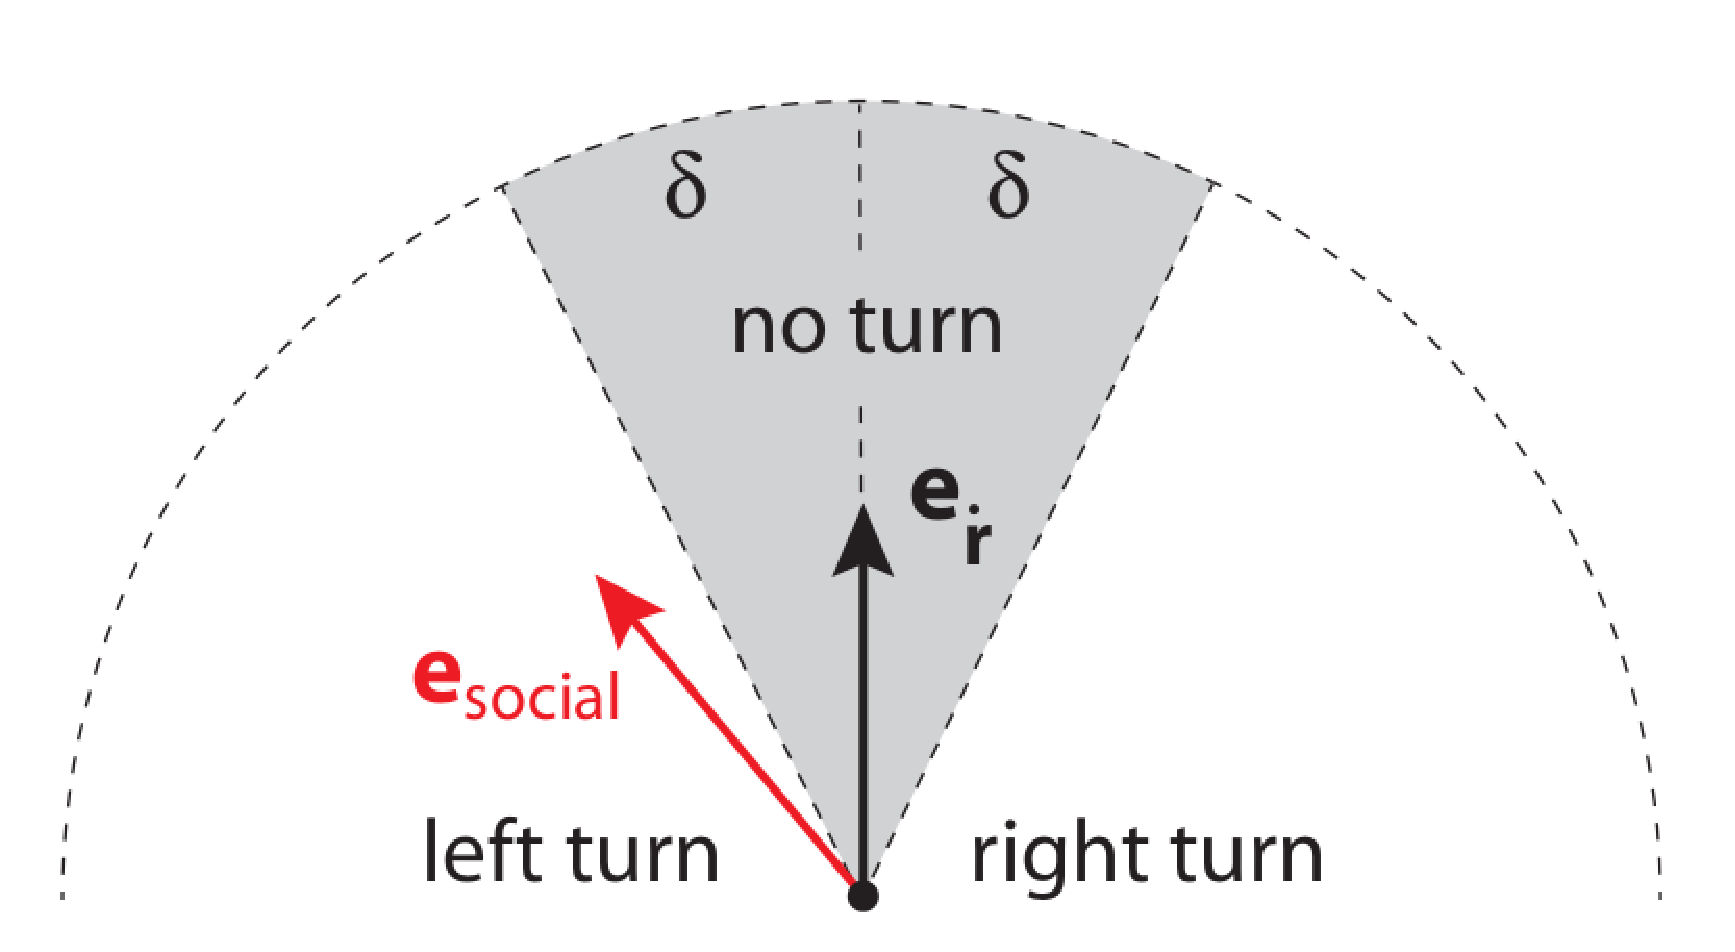
\includegraphics[width=0.4\textwidth]{images/start_turn_pic.eps}
    \caption{(From \cite{hol2012}) When the angle between the current direction of motion $e_{\dot{r}}$ and the desired direction $e_{social}$ is bigger than $\delta$ the skier performs a turn to adjust his or her direction}\label{start_turn_pic}
  \end{center}
\end{figure}

To describe the social force that attracts the skier towards the chosen destination, the model assumes that each skier, while descending, selects several waypoints $x_a^1....x_a^n$ as temporary destinations. Thus, at each time $t$ the skier $a$ wants to reach a waypoint $x_a^k$. The direction toward the current waypoint is expressed by

\begin{equation}\label{waypoint_direction}
e_a(t)=\frac{x^k_a-r_a(t)}{\Vert x^k_a-r_a(t) \Vert}
\end{equation}
where, as defined above, $r_a(t)$ is the position of $a$ at time $t$. The destination social force drives the skier toward the waypoint and is defined as

\begin{equation}\label{destination_force}
F_D(r_a)=A_0 e_a(t)
\end{equation}
where $A_0$ is a scaling constant that represents the strength of the destination force.

The attitude of skiers to keep a minimum distance from the edges is modeled with repulsion forces that are stronger when the skier gets closer to the edge of the slope. At each position $r_a$ the skier $a$ is subjected to repulsion forces from the left and right edges of the slope. Let $r_a^L$ be the closest location to $r_a$ on the left edge, then the distance between the skier and the edge can be expressed as $r_{aL}=r_a-r_A^L$. The repulsion force from the left edge is defined as

\begin{equation}\label{left_force}
F_L(r_{aL})=-\nabla_{r_{aL}}U(\Vert r_{aL} \Vert )
\end{equation}
where $U(\Vert r_{aL} \Vert )$ is a monotonically decreasing potential. In a symmetric way the repulsion force from the right edge can be defined as

\begin{equation}\label{right_force}
F_R(r_{aR})=-\nabla_{r_{aR}}U(\Vert r_{aR} \Vert )
\end{equation}

The model takes into account also the natural human behavior of avoiding collisions with other skiers. This is described by a repulsion force, referred as skier repulsion force, that each skier imposes on the other skiers. The repulsion force that skier $b$ imposes on the skier $a$ can be expressed as

\begin{equation}\label{skier_force}
F_S(r_{ab})=-\nabla_{r_{ab}}V(s(r_{ab}))
\end{equation}
where $r_{ab}=r_a-r_b$ is the distance vector between the two skiers, $V(s(r_{ab}))$ is a monotonically decreasing potential with equipotential lines shaped as ellipses directed into the direction of motion and $s$ represents the semiminor axis of this ellipse and is defined as

\begin{equation}\label{skier_s}
s(r_{ab})=\frac{\sqrt{(\Vert r_{ab} \Vert + \Vert r_{ab}-v_b \Delta t e_b \Vert )^2-(v_b \Delta t)^2}}{2}
\end{equation}

Finally a repulsion force from the obstacles on the slope is considered. The force that an obstacle $o$ imposes on the skier $a$ is defined as

\begin{equation}\label{obstacle_force}
F_O(r_{ao})=-\nabla_{r_{ao}}W(\Vert r_{ao} \Vert )
\end{equation}

In general, repulsion social forces act on skiers only if he or she is capable of perceiving what triggers the force. The model assumes that objects are perceived only within a certain range $\varphi$ of the skier direction. $2\varphi$ can be considered as the angle of view. This is modeled by the weight

\begin{equation}\label{visibility}
w(u,v)=\begin{cases}
  1 & \text{if $(u/\Vert u \Vert)\cdot (v/\Vert v \Vert) \geq cos \varphi$} \\
  0 & \text{otherwise }
  \end{cases}
\end{equation}

To summarize, social forces modeled for every skier $a$ are
\begin{align}\label{social_forces_tb}
F_D(r_a)&=A_0 e_a(t),\\
F_L(\dot{r_a},r_{aL})&=w(\dot{r_a},-r_{aL})F_L(r_{aL}),\\
F_R(\dot{r_a},r_{aR})&=w(\dot{r_a},-r_{aR})F_R(r_{aR}),\\
F_A(\dot{r_a},r_{ab})&=w(\dot{r_a},-r_{ab})F_A(r_{ab}),\\
F_O(\dot{r_a},r_{ao})&=w(\dot{r_a},-r_{ao})F_O(r_{ao})
\end{align}

The resultant social force $F^a_{social}$ is the superposition of all social forces that apply on skier $a$:

\begin{equation}
F^a_{social}=F_D(r_a)+F_L(\dot{r_a},r_{aL})+F_R(\dot{r_a},r_{aR})+\sum_b F_A(\dot{r_a},r_{ab})+\sum_o F_O(\dot{r_a},r_{ao})\nonumber
\end{equation}
Figure \ref{social_forces_diagram} shows a diagram of the social forces described above.

\begin{figure}[!ht]
  \begin{center}
    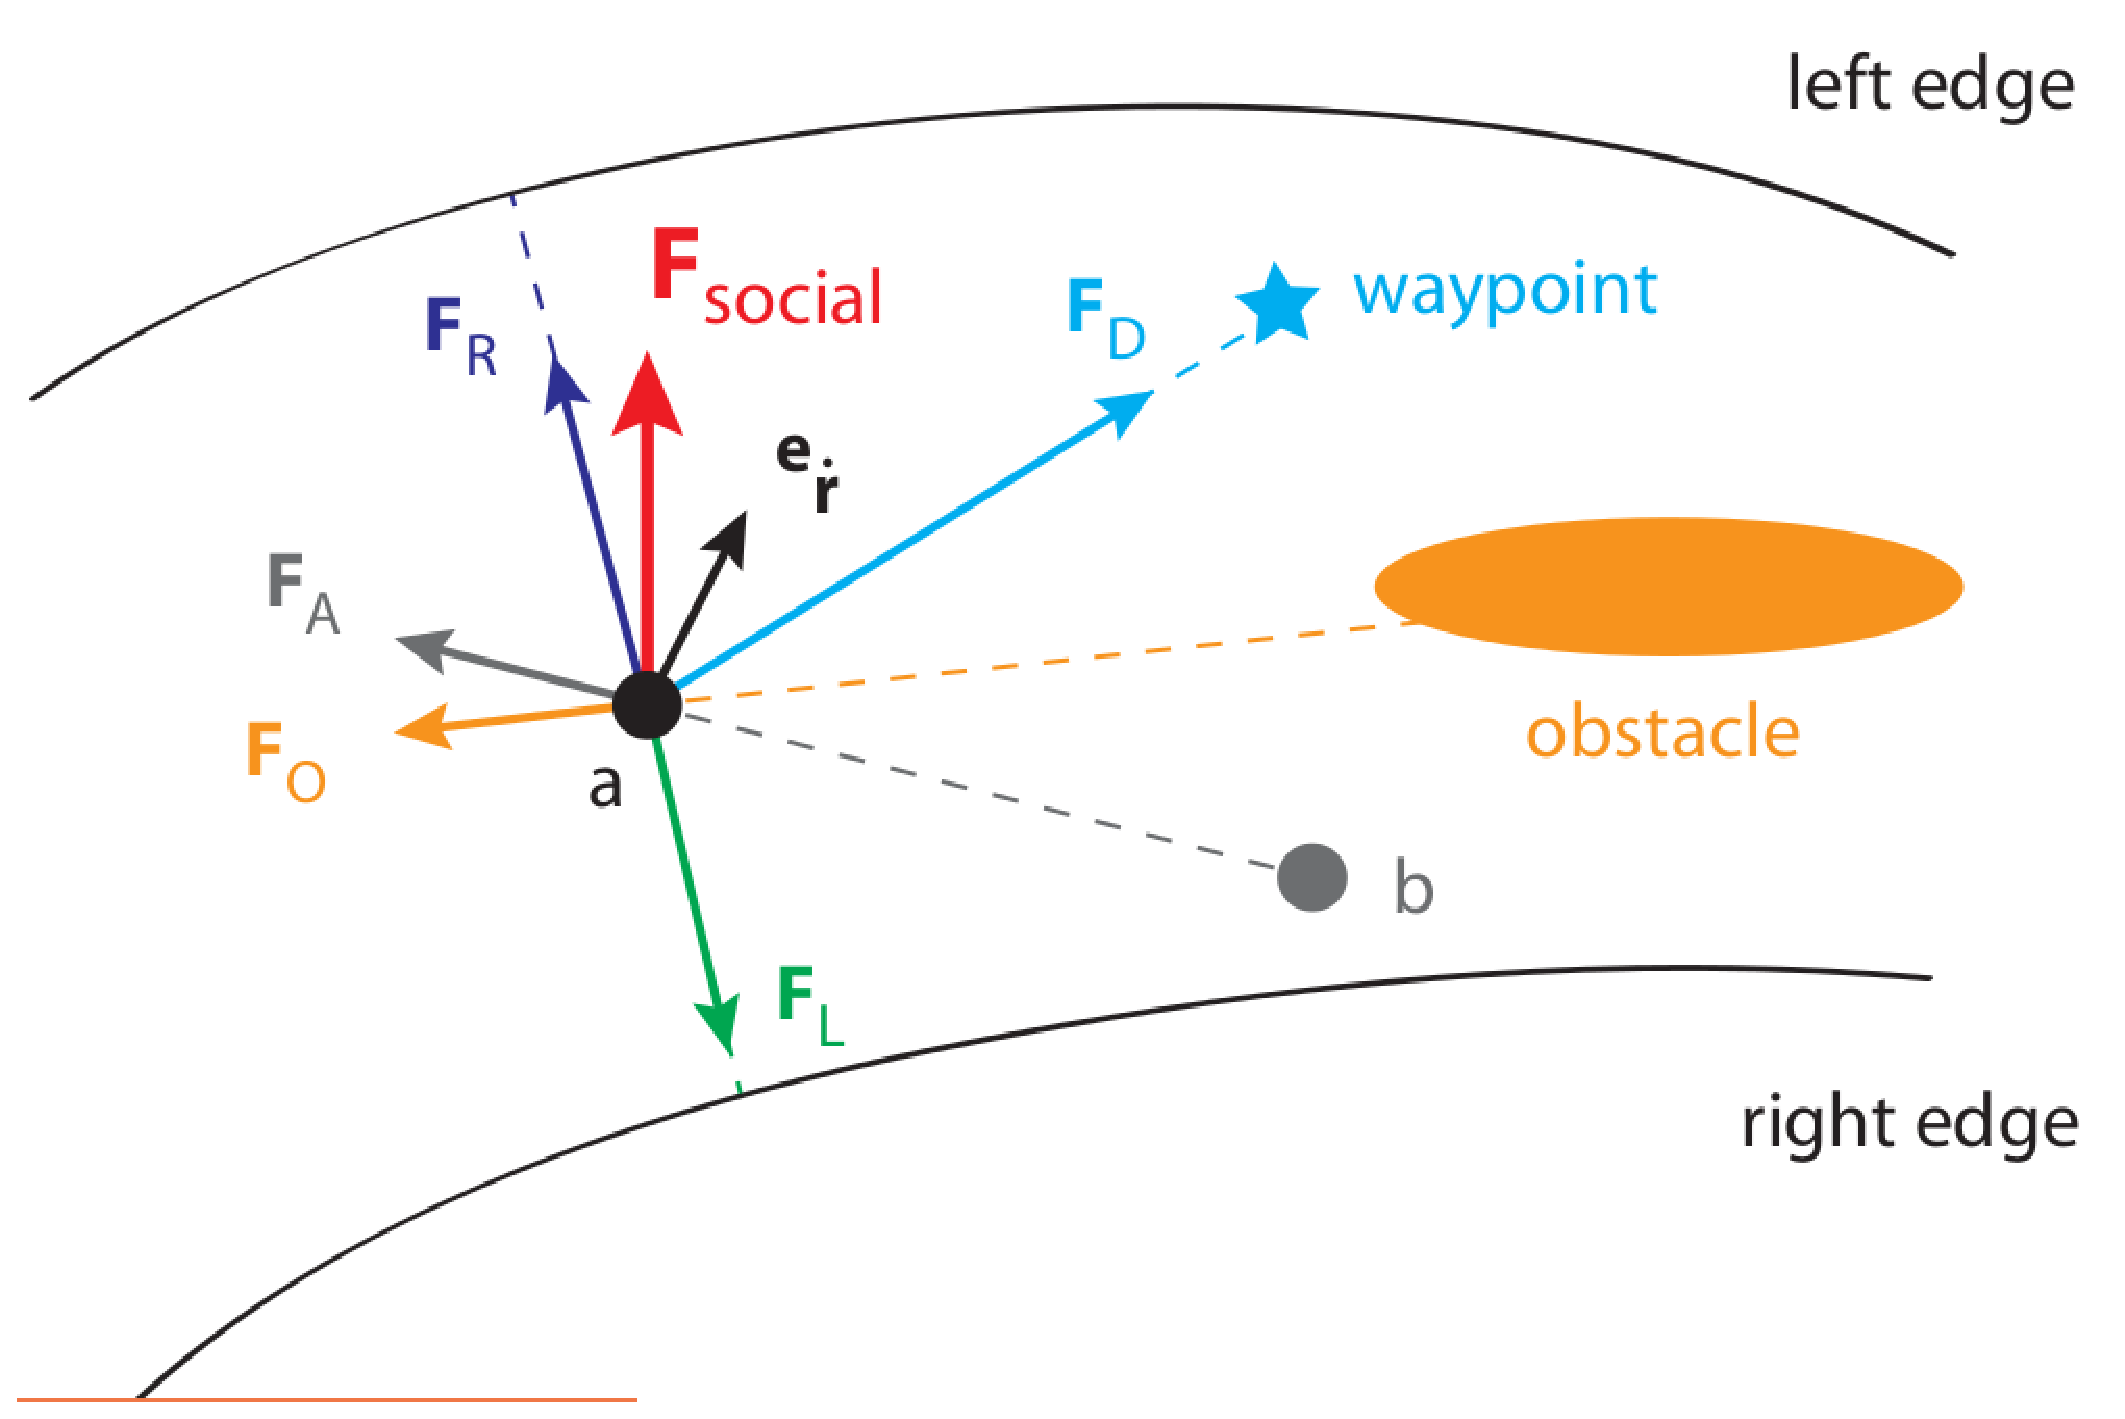
\includegraphics[width=0.8\textwidth]{images/social_forces_dia.eps}
    \caption{Diagram of the social forces. The forces $F_R$ and $F_L$ keep the skier $a$ away from the edges, the force $F_O$ repels the skier from the obstacle, the force $F_S$ repels $a$ from the skier $b$ and the force $F_D$ attracts the skier towards the waypoint.}\label{social_forces_diagram}
  \end{center}
\end{figure}


\section{Physical forces}
As described in \cite{hol2012}, there are two major techniques used to curve while skiing: \textit{skidding} and \textit{carving}. When carving, the direction of motion is exclusively parallel to the skis while in skidding there is an additional slippage to the side. Carved turns are usually performed by expert skiers, while beginners and non-experienced skiers tend to perform skidded turns.

In \cite{hol2012} skiers are supposed to perform turns with a radius corresponding to the \textit{sidecut radius} of their skis. Although some studies \cite{jen2004} \cite{fe2010} have proposed a more realistic model of carving turns,deeply investigating the effects of ski penetration in the snow and of the skier tilt angle, as a first version of the model the approximation of the turning radius to the sidecut radius has been considered acceptable. Figure \ref{sidecut_radius} shows the relation between sidecut radius and turning radius.

\begin{figure}[!ht]
  \begin{center}
    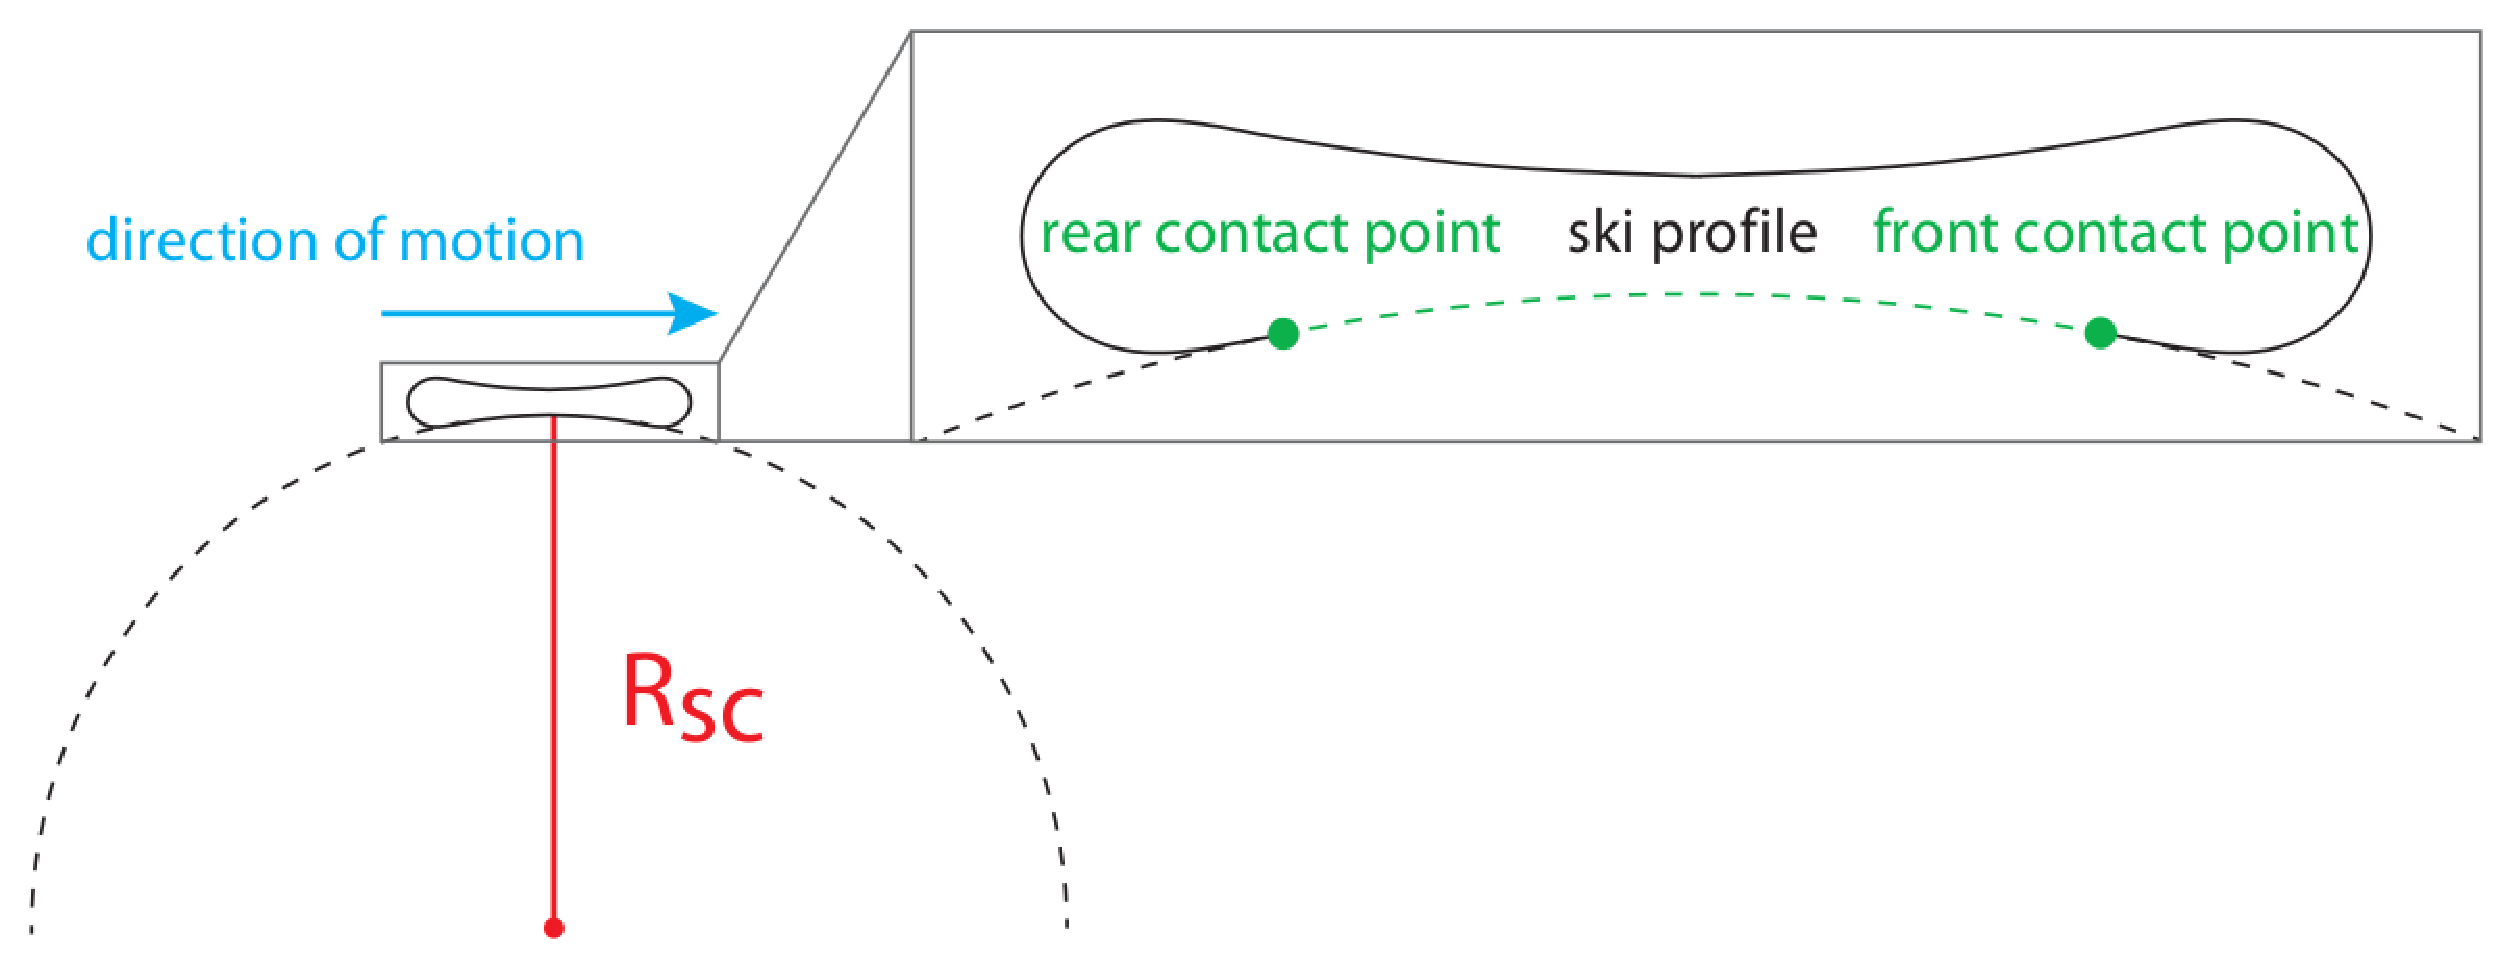
\includegraphics[width=0.8\textwidth]{images/sidecut_radius.eps}
    \caption{(from \cite{hol2012}) Profile of a carving sking with the sidecut radius and the turning radius evidenced.}\label{sidecut_radius}
  \end{center}
\end{figure}

Gravitational, centripetal and friction forces determine the skier acceleration according to their direction $e_{\dot{r}}$. Consider a skier at position $r$ with speed $\dot{r}$ and direction of motion $e_{\dot{r}}$ and let $n$ denote the surface normal on the ski slope at $r$. At $r$, the slope has an inclination angle of

\begin{equation}
\alpha =\arccos(\left[0,0,1\right] \cdot n)
\end{equation}
and the inclination angle $\gamma$ of the current trajectory $e_{\dot{r}}$ is

\begin{equation}
\gamma =\arcsin[(\sin \alpha )(\sin \beta )]
\end{equation}
where $\beta$ is the angle between $e_{\dot{r}}$ and the horizontal of the slope.

To compute the force accelerating the skier the gravitational force, the friction forces and the centripetal forces should be investigated. As first the gravitational force $F_G$ is considered. It can be expressed as

\begin{equation}
F_G=mg\left[\begin{matrix}0\\0\\-1\end{matrix}\right]
\end{equation}
where $g$ is the gravitational acceleration and $m$ the mass of the skier. The gravitational force can be subdivided into normal force $F_N$, acting parallel to the surface normal $n$, and into downhill force $F_S$, acting parallel to the fall line.

\begin{equation}\label{downhill_force}
F_G=F_S-F_N
\end{equation}
The normal force $F_N$ can be expressed as
\begin{equation}
F_N=mg(\cos \alpha )n
\end{equation}

The  downhill force $F_S$ itself can be subdivided into $F_P$ which is acting parallel to the current trajectory $e_{\dot{r}}$ and into the lateral force $F_{lat}$ acting perpendicularly to the current trajectory (see. Fig\ref{downhill_force_pic}).

\begin{equation}
F_S=F_P+F_{lat}
\end{equation}
\begin{figure}[!ht]
  \begin{center}
    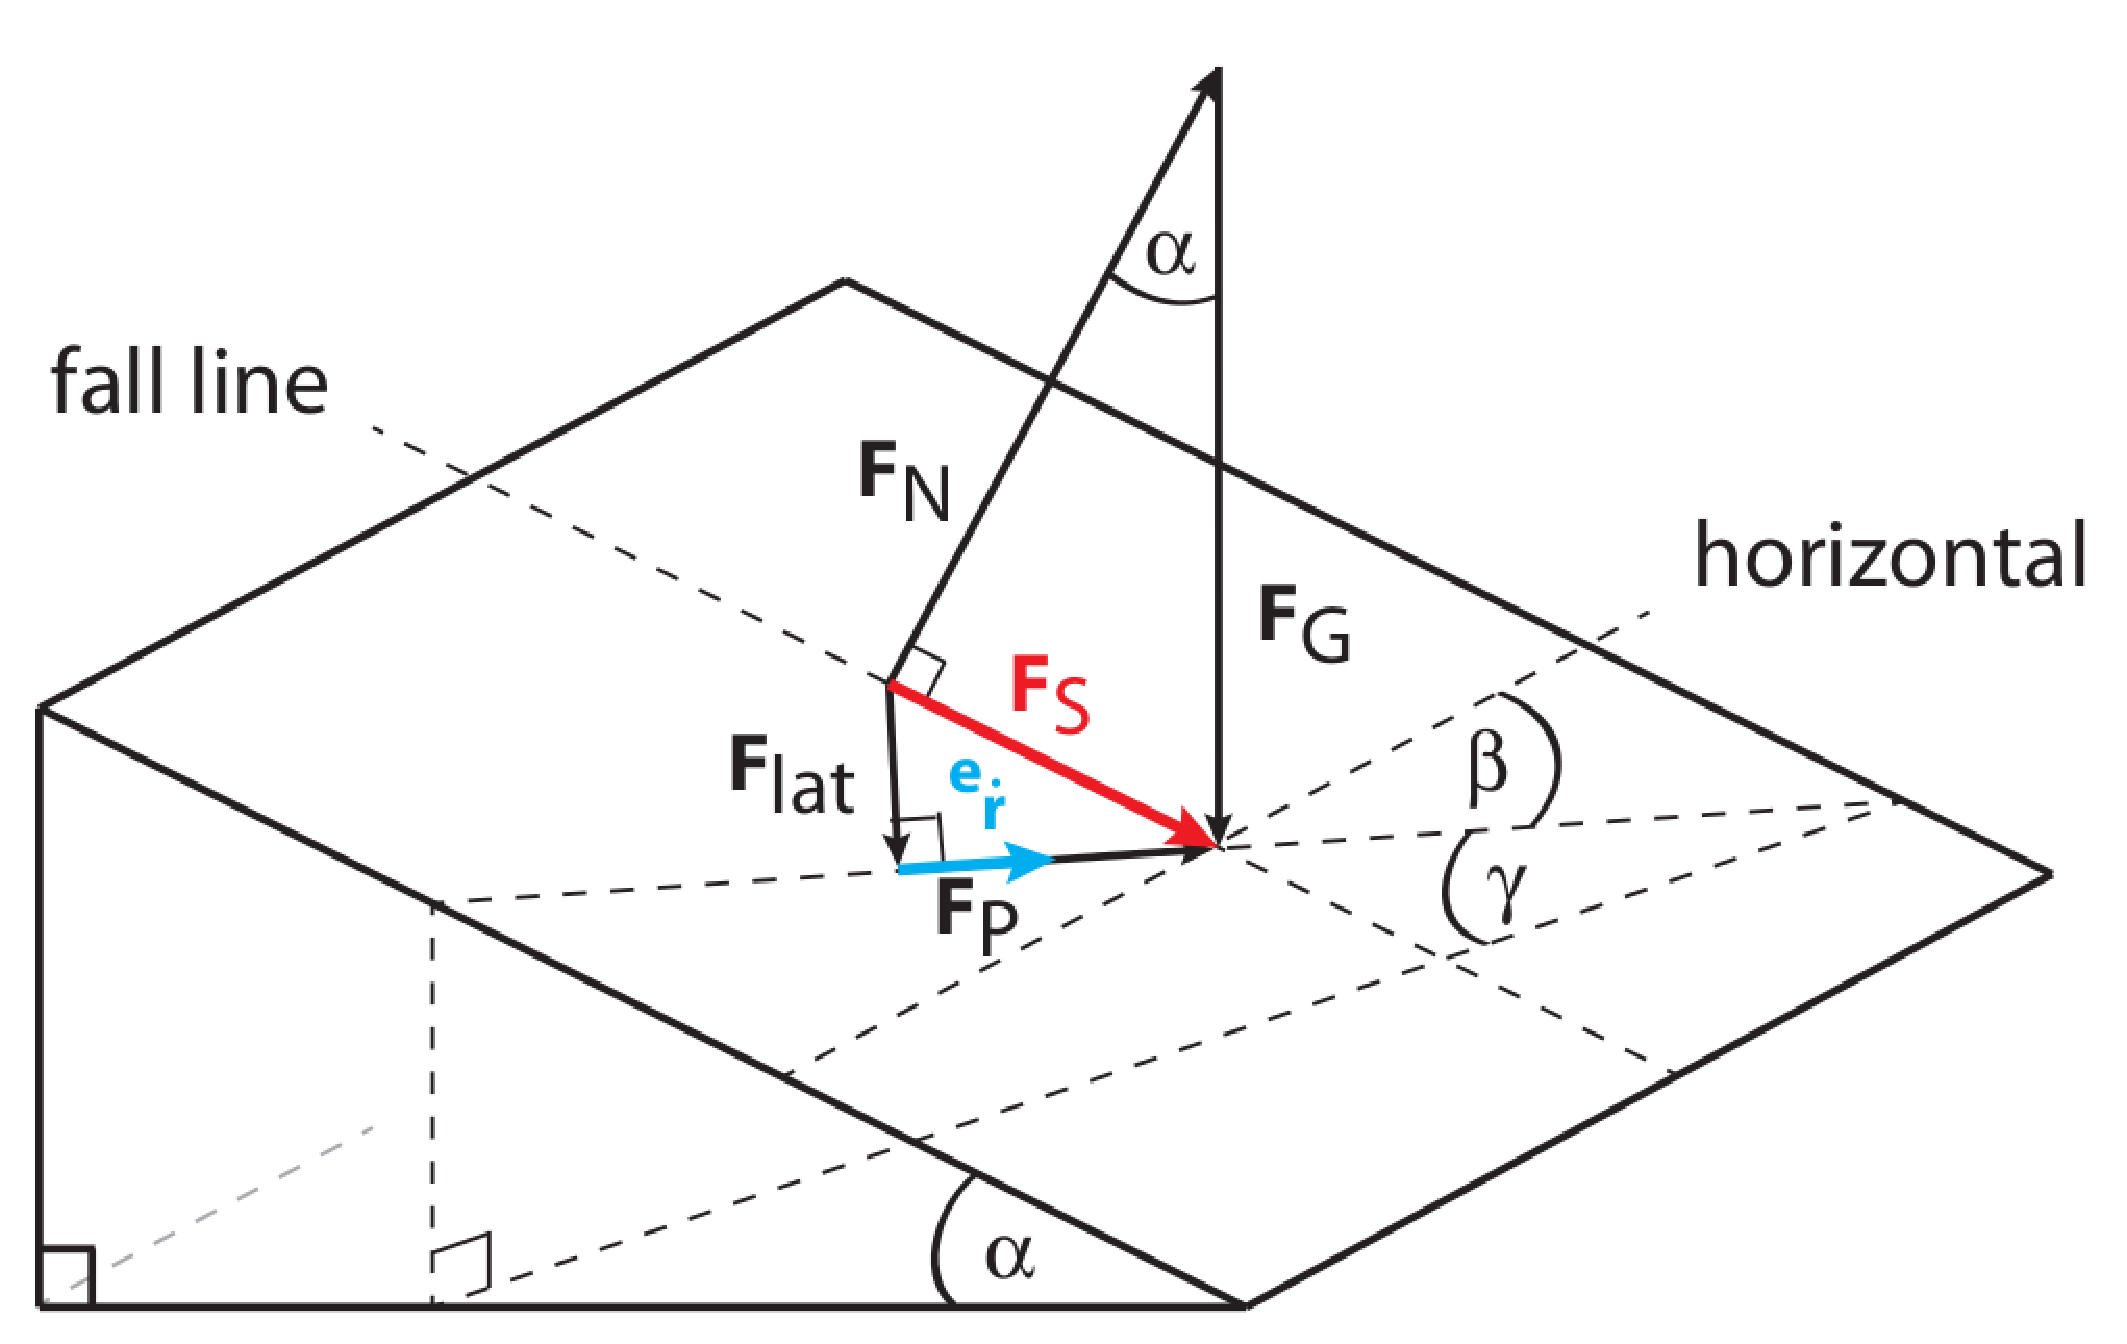
\includegraphics[width=0.5\textwidth]{images/figure5.eps}
    \caption{(from \cite{hol2012}) The downhill force $F_S$ can be decomposed into the downhill force $F_P$, acting parallel to the current trajectory, and into the lateral force $F_{lat}$ acting perpendicularly to the direction of travel.}\label{downhill_force_pic}
  \end{center}
\end{figure}

The downhill force $F_p$ can be written as
\begin{equation}
F_P=mg ( \sin \gamma ) e_{\dot{r}}=mg ( \sin \alpha ) ( \sin \beta ) e_{\dot{r}}
\end{equation}
where $\gamma$ is the inclination angle of $e_{\dot{r}}$.

Remembering \ref{downhill_force}, the downhill force $F_S$ can be computed as
\begin{equation}
F_S=F_G+F_N
\end{equation}
The lateral force $F_{lat}$ can therefore be computed as

\begin{equation}
F_{lat}=F_S-F_P
\end{equation}
The centripetal force $F_C$ a skier is exposed while turning can be written as

\begin{equation}
F_C=\frac{m}{R_{SC}} {\norm{\dot{r}}}^2 \frac{F_{lat}}{\norm{F_{lat}}} \times
\begin{cases}
  (+1) & \text{before crossing the fall line} \\
  (-1) & \text{after crossing the fall line}
  \end{cases}
\end{equation}
where $m$ is the mass of the skier and $R_{SC}$ the sidecut radius of the skis. $F_C$ is parallel to $F_{lat}$ before the skier crosses the fall line and antiparallel to $F_{lat}$ after having crossed the fall line.

Before defining the kinetic friction of skis on snow, a definition of effective force should be given. The effective force is the force that needs to be compensated by the snow. Its formulation depends on whether the skier is performing a turn or is descending on a straight line. In the following, when the definition of a force changes depending on whether the skier is turning, the index is written lowercase in the case of a straight line and uppercase in the case of a turn. So $F_{eff}$ is the effective force acting on a skier that is descending on a straight line and is defined as

\begin{equation}
F_{eff}=F_{lat}-F_N
\end{equation}
If the skier is performing a carved turns then the effective force $F_{EFF}$ can be written as

\begin{equation}
F_{EFF}=F_{lat}-F_C-F_N
\end{equation}
Figure \ref{effective_force_pic} shows the effective force ($F_{eff}$ and $F_{EFF}$).

\begin{figure}[!ht]
  \begin{center}
    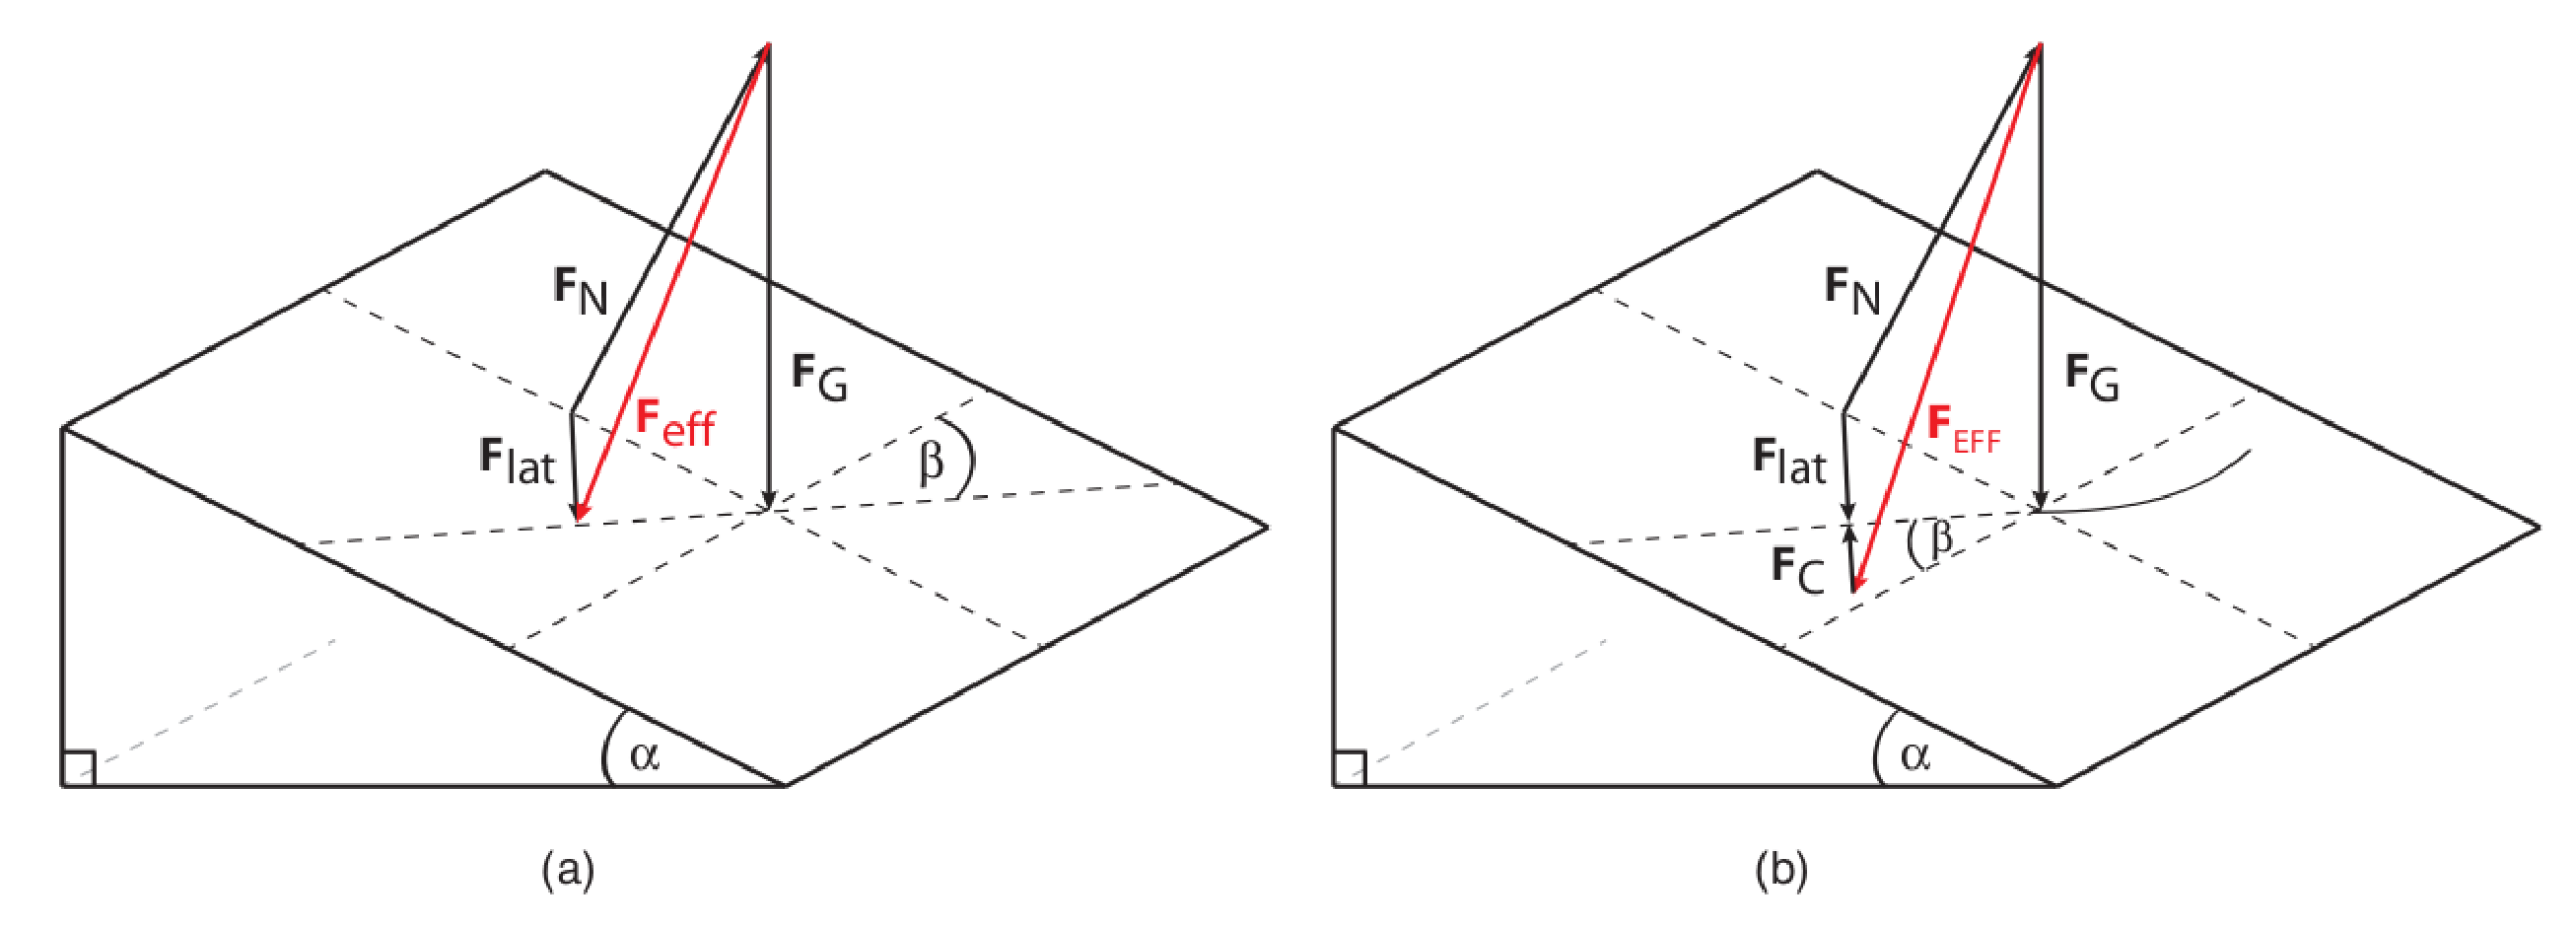
\includegraphics[width=\textwidth]{images/figure6.eps}
    \caption{(from \cite{hol2012}) In (a) effective force during the descent on a straight line ($F_{eff}=F_{lat}-F_N$). In (b) effective force during a carved turn ($F_{EFF}=F_{lat}-F_N-F_C$)}\label{effective_force_pic}
  \end{center}
\end{figure}

The kinetic friction force $F_{ground}$ can be expressed in terms of the skier's effective force as

\begin{equation}
F_{ground}=-\mu \norm{F_{eff}}e_{\dot{r}}
\end{equation}
when descending on a straight line. $\mu$ is the kinetic friction coefficient of the skis on the snow. In case of a turn

\begin{equation}
F_{GROUND}=-\mu \norm{F_{EFF}}e_{\dot{r}}
\end{equation}

The air drag force $F_{air}$ is antiparallel to the direction of motion $e_{\dot{r}}$ and is defined as

\begin{equation}
F_{air}=-\frac{1}{2}C_d \rho A \norm{\dot{r}}^2 e_{\dot{r}}
\end{equation}
where $C_d$ is the drag coefficient, $\rho$ the air density and $A$ the projected frontal area of the skier perpendicular to the direction of motion.

Finally, the net force $F_{net}$ accelerating the skier can be defined as

\begin{equation}
F_{net}=-F_P + F_{air} + F_{ground}
\end{equation}
if the skier is not turning. Otherwise the force is defined as

\begin{equation}
F_{NET}=-F_P + F_{AIR} + F_{GROUND} + F_C
\end{equation}

\section{Limitations}
The model proposed describes the motion of an expert skier that skies performing perfect carved turns and the turning radio is taken constant and equals to the sidecut radius of the skis. Not experienced skiers and other snow-sport athletes are not considered. An important limitation of the model is that it does not consider that skiers could stop while descending a slope.  Moreover skiers are not allowed to jump nor to exit the ski slope. If a skier collides with an edge of the slope it is reflected back with an angle equals to the angle at which he or she has collided.

\section{Differences from the original model}
The physical model of the skiers motion is identical to the one exposed in \cite{hol2012}. Within the social forces, the destination force $F_D$ (see. \ref{destination_force}) is of critical importance. The effectivness of this destination force is strongly related to the waypoints selection. In the original paper the waypoints were selected randomly every 50m, using a uniform distribution on the corresponding line from the left to the right edge of the slope (see Fig.\ref{waypoints_old_pic}).

\begin{figure}[!ht]
  \begin{center}
    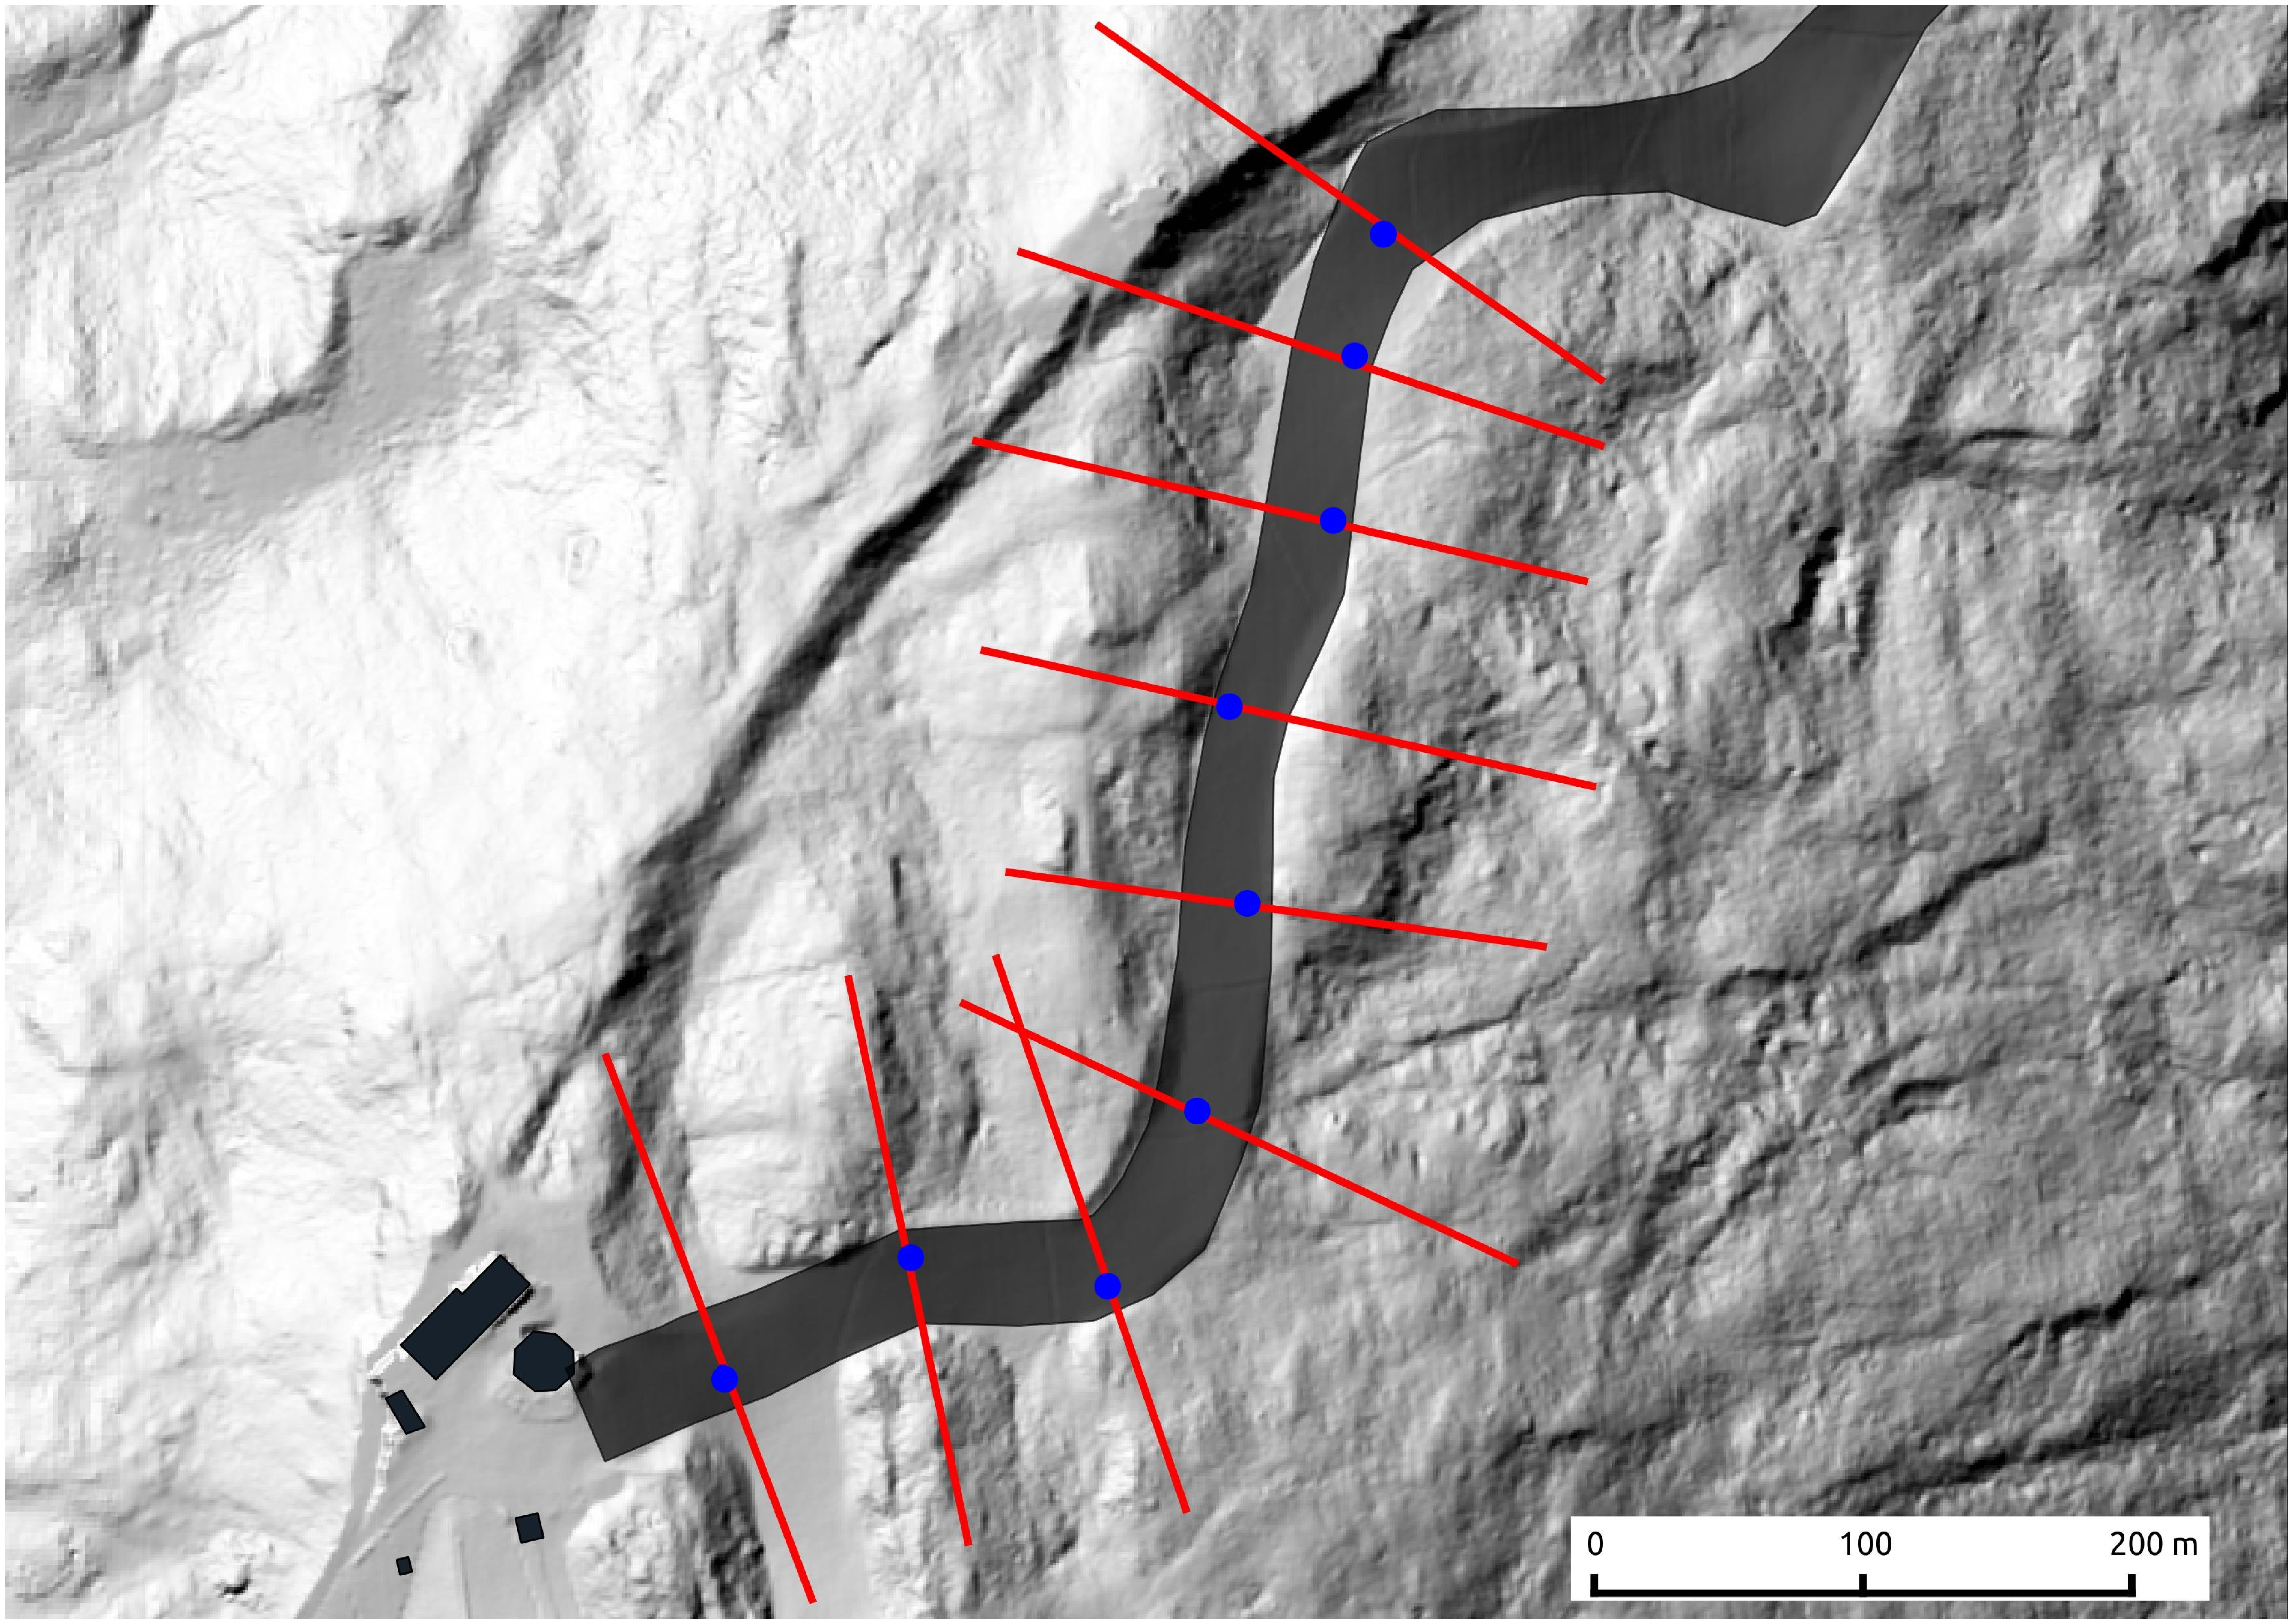
\includegraphics[width=\textwidth]{images/waypoint_line.eps}
    \caption{In \cite{hol2012} waypoints were selected randomly every 50m following a uniform distribution on the line from the left to the right edges of the slope.}\label{waypoints_old_pic}
  \end{center}
\end{figure}

A more dynamic approach in the waypoints selection has been considered to better model the decisions taken from a skier while descending a slope. The new strategy allow each skier to dynamically choose waypoints during the descent, based on the position of the skier, on the shape of the trail, on the slope of the terrain and on the skier speed.

Hereafter the new mechanism for the waypoints selection is explained. Let $a$ be a skier at position $r_a$, let $r_a^L$ be the location on the left slope edge closest to $r_a$ and $r_a^R$ the location on the right slope edge closest to $r$. The vectors given the direction toward the edges are $e_{aR}=\left(r_a^L-r_a\right)/\norm{r_a^L-r_a}$ and $e_{aL}=\left(r_a^R-r_a\right)/\norm{r_a^R-r_a}$. Let $\alpha$ be the angle between $e_{aR}$ and $e_{aL}$ defined as

\begin{equation}
\alpha=\begin{cases}
  \arccos(e_{aR} \cdot e_{aL}) & \text{if(($e_{aR} \times e_{aL})\cdot n \ge 0$)} \\
  2\pi-\arccos(e_{aR} \cdot e_{aL}) & \text{if(($e_{aR} \times e_{aL})\cdot n < 0$)}
\end{cases}
\end{equation}
where $n$ is the normal of the plane containing $e_{aR}$ and $e_{aL}$. The skier $a$ chooses the new waypoint with uniform distribution on a fraction of the angle $\alpha$. More precisely, let $\delta$ be the fraction of angle that should be considered, then the new waypoint $w_a$ is chosen as

\begin{equation}\label{new_waypoint}
w_a=r_a+\rho F\left(\frac{e_{aR}+e_{aL}}{\norm{e_{aR}+e_{aL}}},\mathcal{U}\left(-\frac{\alpha\delta}{2},\frac{\alpha\delta}{2}\right)\right)
\end{equation}
where $\rho$ is the distance at which waypoint are chosen, $F\left(v,\beta\right)$ rotates the vector $v$ of an angle $\beta$ and $\mathcal{U}(a,b)$ returns a random number with uniform distribution on $(a,b)$ (see Fig.\ref{new_waypoint_pic}).

\begin{figure}[!ht]
  \begin{center}
    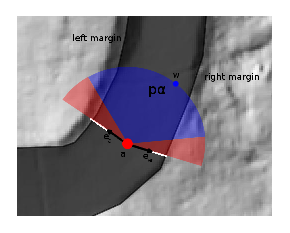
\includegraphics[width=\textwidth]{images/waypoint_new.eps}
    \caption{Selection of a waypoint: the skier $a$ selects the new waypoint $w$ choosing with uniform distribution on the angle $\delta\alpha$, a fraction of $\alpha$. The angle $\alpha$ is the angle between $e_{aR}$, the vector representing the direction towards the right edge, and $e_{aL}$, the vector towards the left edge,}\label{new_waypoint_pic}
  \end{center}
\end{figure}

A new waypoint is selected when the old waypoint is no longer feasible, meaning that it is not in the interval that the skier would consider when choosing a new waypoint, or when the skier has traveled more than $D$ meters after having chosen the last waypoint.

The new approach for waypoints selection considers closely skier speed and the effect of the slope shape on skier's action:\begin{enumerate}
\item \label{depending_velocity} When skiers are faster they tend to turn more often to decrease the speed.
\item \label{frequency} Frequency of the selection of new waypoints should depend on the skiers speed, the more skiers are traveling fast, the more frequently they will choose new waypoints.
\item \label{depending_slope} The selection of a new waypoint should depend on the slope that the skier will face in his range of action: before flat areas skiers tend to go straight to increase velocity.
\item \label{avoid_impact} Skiers usually avoid to choose a direction that would make them turn on the edge of the slope. Therefore, the new waypoint should be in a position that does not lead the skier to impact the edge of the slope.
\end{enumerate}

To model the influences of skier's speed and shape of the slope it is possible to act on the parameter $\delta$ of the equation \ref{new_waypoint}. When $\delta$ is increasing, the width of the angle in which new waypoints can be chosen becomes larger. As a consequence the probability of performing turns becomes higher.

Point \ref{depending_velocity} can be satisfied by making the parameter $\delta$ linearly depend on skier's speed $v$. Moreover it is required that when the speed $v$ is close to $0$ the width of the angle should be also close to $0$ and when $v$ is close to a high value of speed $v_{max}$ the angle should have maximum width. Therefore, $\delta$ can be set to
\begin{equation}\label{delta_vel}
\delta= \frac{v}{v_{max}}
\end{equation}

The requirement \ref{frequency} is already met by the mechanism described above. In fact, since a new waypoint is chosen each time the skier has traveled more than $D$ meters, when a skier is faster he or she chooses waypoints more frequently.

To fulfill the third requirement an additional factor depending on the slope should be considered. Let $s$ be the slope that the skier is going to encounter and let $s_{lim}$ a value of slope that is considered small enough to require an additional acceleration by the skier. Then if $s<s_{lim}$ the width of the angle in which to choose the new waypoint should be narrowed again. Taking into account \ref{delta_vel} then we can write $\delta$ as

\begin{equation}
\delta=\begin{cases}
   \frac{v}{v_{max}}\frac{s}{s_{lim}} & \text{if ($s < s_{lim}$)} \\
   \frac{v}{v_{max}} & \text{otherwise}
\end{cases}
\end{equation}
If, despite this, skiers will come to a complete stop (maybe due to a counter slope), they will start walking at constant speed.

Finally, to satisfy point \ref{avoid_impact} manipulating $\delta$ will not be enough. The minimum turning radius of skiers gives a bound to their ability of avoiding a collision or to hit the edges of the ski slope. Assuming that a skier do not choose a direction that will make them exit the ski slope, those angles indicating a direction along which the slope edge is reached in less than $R_{SC}$ meters are not considered in the selection of the waypoint.

\chapter{Implementation}\label{implementation}
The model was implemented using C++ and GRASS GIS. GRASS GIS is a Geographic Information System (GIS) open source software used for geospatial data management and analysis. It was chosen to perform the geospatial computation needed by the model.

\section{Technology choice}
Different technologies were explored to implement the GIS Backend needed by the model. PostGIS, QGIS, GDAL/OGR and GRASS GIS were the main technologies considered.

PostGIS is an open source spatial database extender for PostgreSQL database. It gives support for geographic objects manipulation allowing spatial queries to be run in SQL. The critical point using PostGIS is the absence of a dedicated API for any language. It requires to use a PostgreSQL adapter (such as psycopg for python) and to build dynamically the queries in the chosen language. Moreover the raster data support is still immature.

Quantum GIS Desktop, also known as QGIS, is an open source GIS desktop application. QGIS supports both vector and raster formats. It have a module, PyQGIS, that supports scripting using the Python language. However, the functionalities implemented are more focused on spatial data visualization and do not give enough support for the analysis operations.

GDAL, Geospatial Data Abstraction Library, is an open source library for geospatial data translation and processing. The related library OGR Simple Feature Library provides a similar capability for simple vector data processing. GDAL exposes API for C,C++ and Python while the more widely used API for OGR is the one for C++. OGR provides also slightly less complete API for C and Python, although they are not really well documented. The main issue using GDAL/OGR is the lack of support for the analysis of vector data: OGR offers useful API to read and write vector data, but analysis such as point linestring distance calculation are not available.

GRASS GIS, commonly referred to as GRASS (Geographic Resource Analysis Support System) is an open source GIS software that gives support for geospatial data management and analysis. To understand how GRASS API works it is necessary to look at the GRASS software structure (see Fig.\ref{grass_structure}. GRASS has a large GIS library, referred to as GRASS GIS Library, at the basis of the software stack. It is divided in two main library: the Raster File Processing library and the Vector File Processing library. It contains also many others library of less importance. The GRASS GIS Library is quite large and implements many basic GIS operation both for raster and vector format. The spatial data are stored in the GRASS map storage with the GRASS specific format. On the top of the GRASS GIS Library are built many modules for raster and vector processing. The modules perform analysis at a higher level, they are executables and can be used directly from the GRASS GUI or from the command line.

\begin{figure}[!ht]
  \begin{center}
    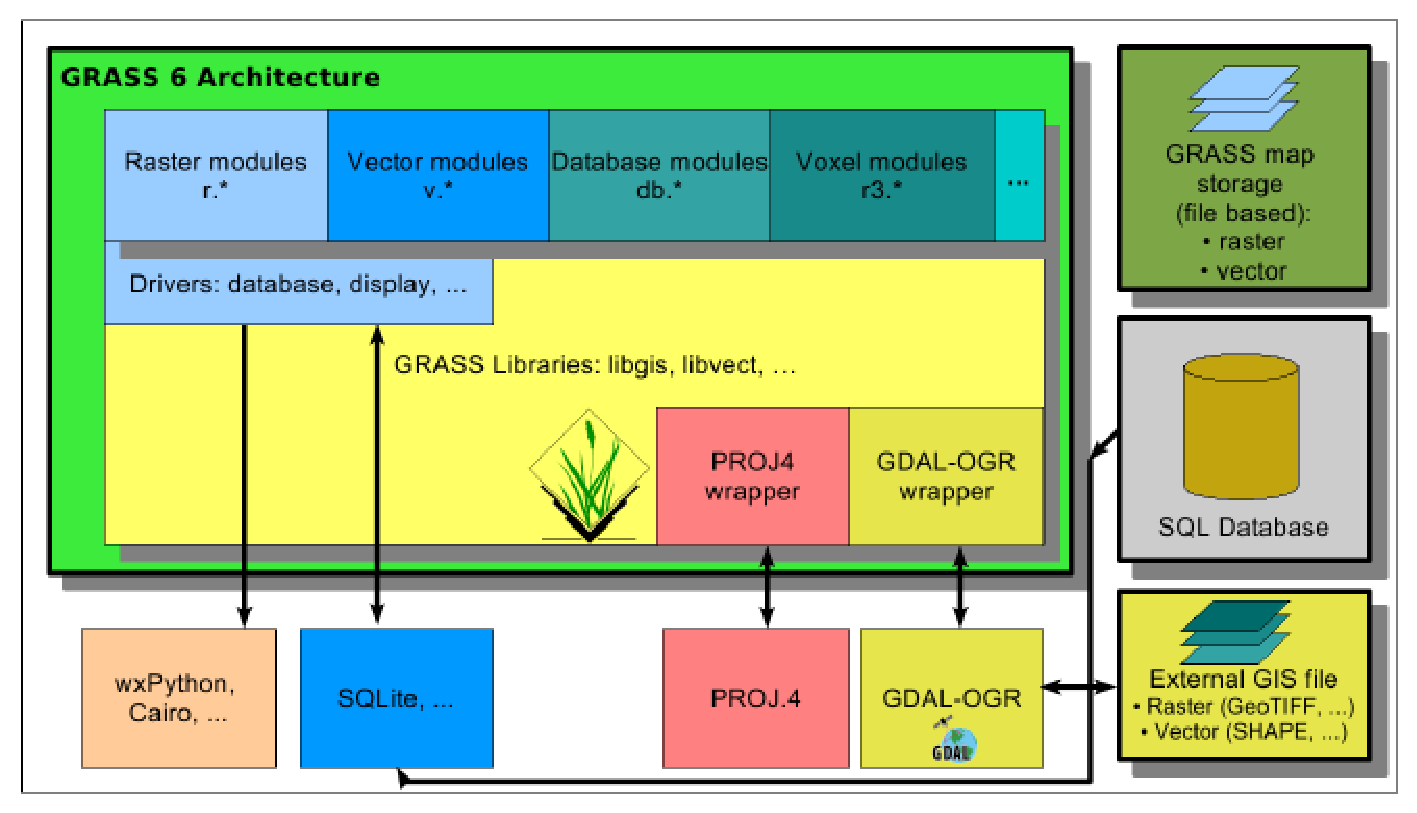
\includegraphics[width=\textwidth]{images/grass6_arch.eps}
    \caption{(from http://grass.osgeo.org} GRASS software architecture\label{grass_structure}
  \end{center}
\end{figure}

GRASS allows two basic levels of programming. The most simple approach is to use script programming to call the high-level GRASS modules. A more advanced approach is to access the low-level functionalities of the GRASS GIS library trough the C-API exposed. Since grass modules are executables, the first approach requires to spawn a new process each time a spatial computation is needed. For the implementation of the model presented in \ref{model} this is not feasible. Even if the second approach forces to use GIS operations at a lower lever it has many advantages: it gives support for database routines (GRASS file management), for projections, for raster and  vector data management and it guarantees good performances \cite{net2008}.

GRASS GIS was chosen to implement the GIS Backend. Since the API is written in ANSI C, writing the code in C or in C++ has the advantage of accessing the API in a very simple manner. Moreover both C and C++ guarantee good performances and are often chosen to implement this kind of simulation. C++ was preferred to C because it is object oriented. An object oriented design allows to better represent the concepts presented in the model, reducing the complexity and making the code structure clearer. Moreover it keeps the code structure more modular and flexible.

\section{Software structure}
The software structure was designed to be the most flexible as possible. The main entities modeled inside the software are the slope, the skiers and the forces. In Figure \ref{class_diagram} the class diagram of the software is described. The class Slope models the ski slope, it has a set of skiers, the skiers that are descending the slope, a set of physical forces, the physical forces that act on the slope and a set of social forces, the social forces skiers are subjected to. The Skier class models a skier: it has a position, a velocity, an acceleration and a status describing if he is turning. The forces have been modeled with two different classes: the SocialForce class and the PhysicalForce class are abstract classes that act as base class respectively for all the social forces and for all the physical forces. Although the interface declared by this two classes is the same, they were not merged together because the two type of forces, social and physical, are conceptually different and in future development it is possible that changes in the model will require to have separated interfaces.

\begin{figure}[!ht]
  \begin{center}
    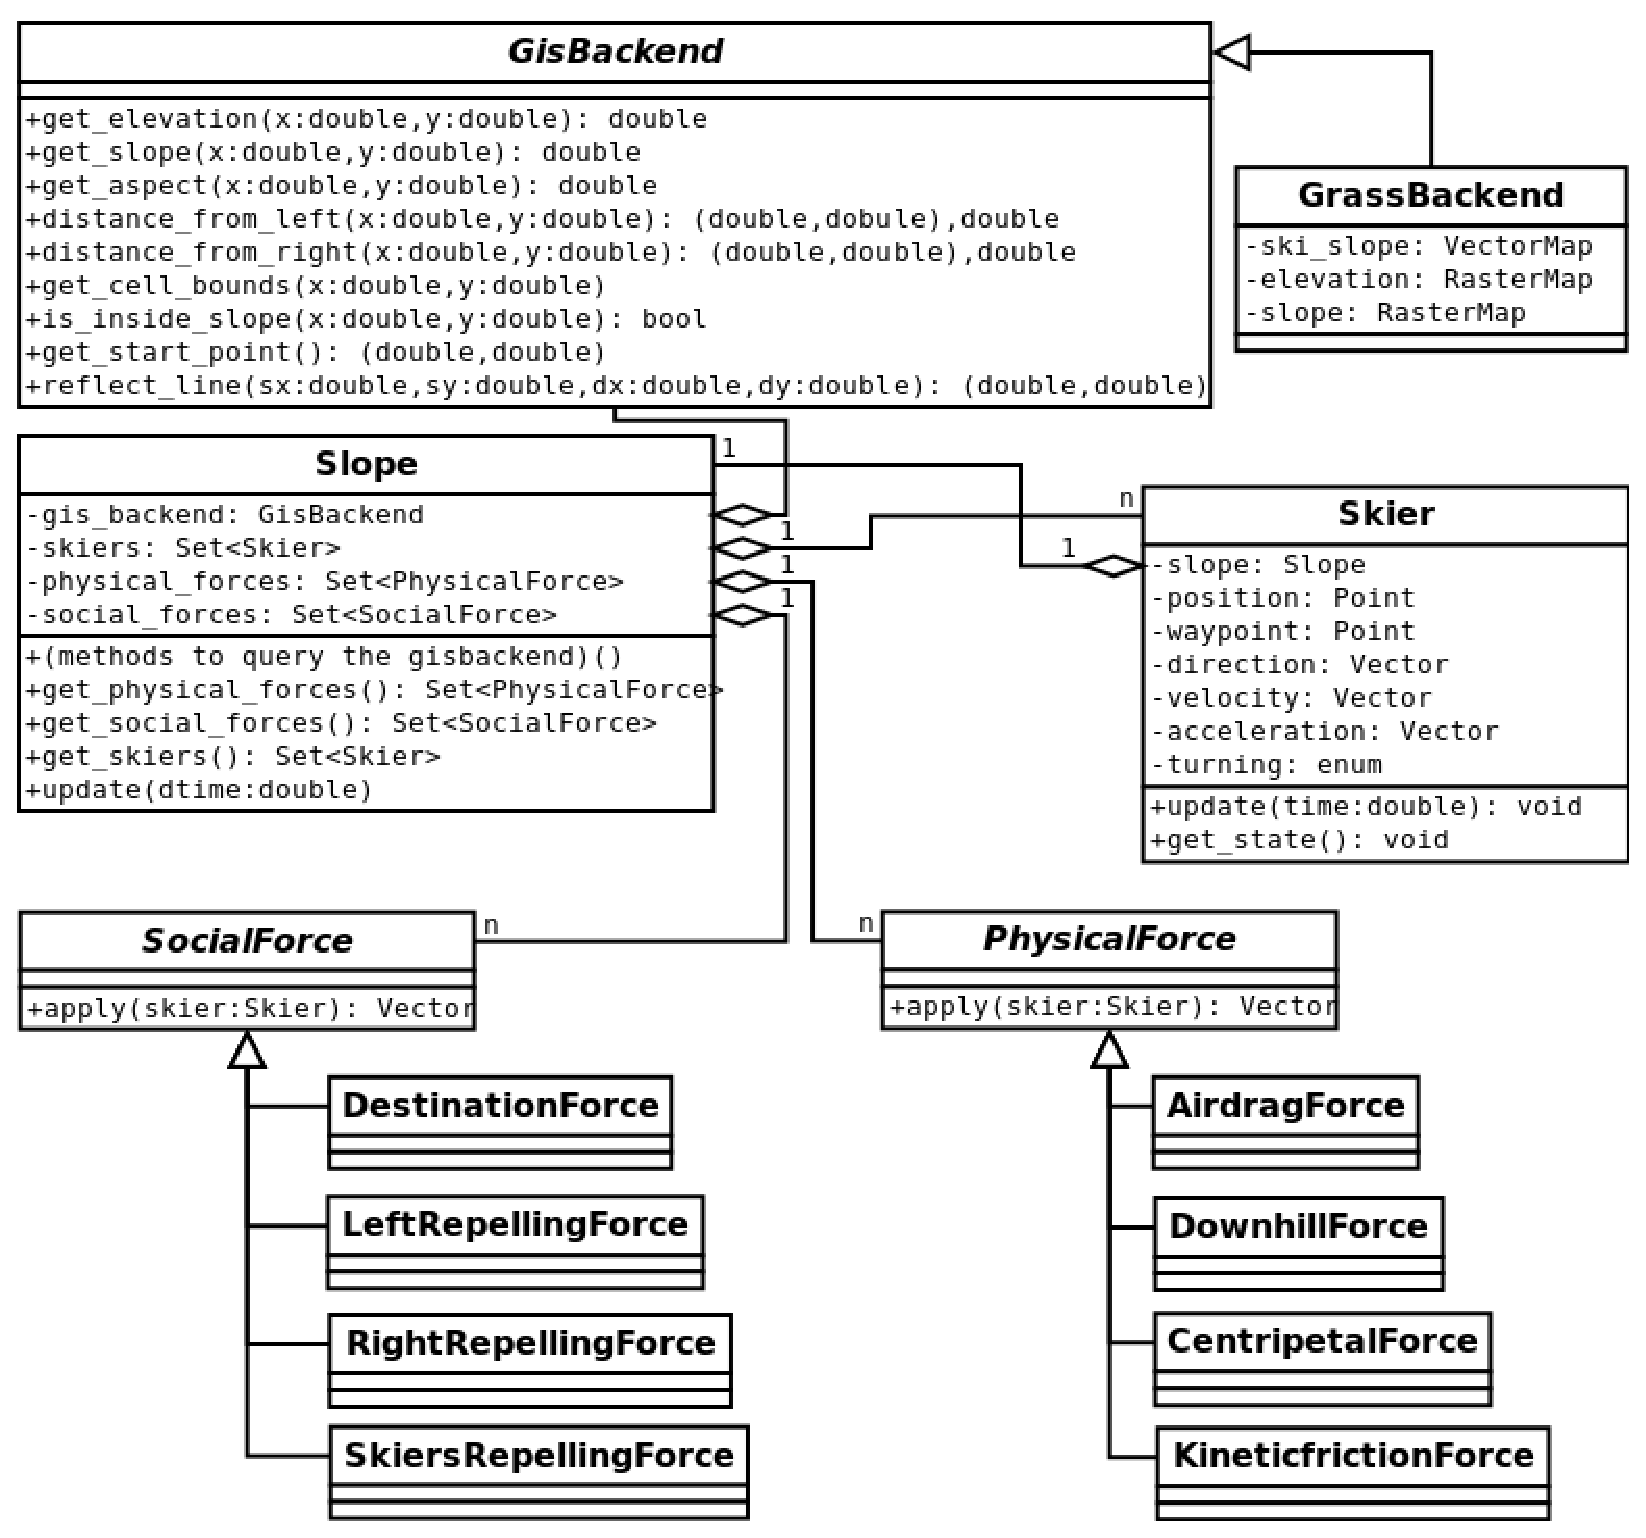
\includegraphics[width=\textwidth]{images/Class_diagram.eps}
    \caption{Class diagram}\label{class_diagram}
  \end{center}
\end{figure}

The simulation has to perform some specific GIS computation. The implementation realized wanted to avoid dependencies between the code related to the simulation and the code written to implement GIS specific operations. In other words the implementation of the simulation should be independent by the technology chosen to implement the GIS Backend. For this reason, an abstract class called GisBackend was used. This class declares the interface that a GIS backend used to run the simulation must implement. This interface includes methods to get elevation, slope and aspect for given coordinates, methods to get the distance of a point from the edges of the slope, methods to give random start points at the top of the ski slope, to determine if a given point is inside the ski slope and a method to reflect a line colliding on a slope edge.

The class GrassBackend implements the interface GisBackend and is the class used in the code when spatial computations are needed. The class GrassBackend performs the operations needed using the GRASS GIS Library. It requires to have available a DEM (Digital Elevation Model) raster map for the elevation and the slope and aspect computation, a vector map with the polygon of the ski slope to determine if a point is inside the slope, a vector map with the lines of the right and left edges of the slope to find the distances from them and finally a vector map with the polygon of the start area and stop area to decide where skiers should be started and stopped.

\section{Input data}
The input data required by the simulation to run are the data needed by the GrassBackend. The Digital Elevation Model used was a Digital Terrain Model (DTM) of the area of Trentino. The DTM was obtained using the LIDAR technology, a remote sensing sensing technology that uses laser light to measures distances. The measurements were done in the years 2006 and 2007. It is at a resolution of 1x1m except for areas at high elevation where resolution is of 2x2m.

The measurements for the DTM were done in seasons without snow. As a consequence the DTM on which real skiers move is different from the DTM obtained with the Lidar. Two strategy was thought to simulate the effect of the snow on the DTM.

The first strategy uses a simple model to simulate the distribution of the snow. The model considers two limit cases to describe the profile of the snow. Given a surface $y(x)$ and a snowfall of $h$ meters, the first case describes a new profile were the snow is supposed to adhere perfectly to the terrain: $y_s(x)=y(x)+h$. The second case considers the snow to behave like a liquid and creates a new profile $y_L(x)$ where the new precipitation accumulates in the valleys, making the profile constant, and leaves $y_L(x)=y(x)$ on the ridges. Neither the first nor the second case can be considered realistic, however it can be thought that the real behavior of the snow can be described as an average between the two cases. So the actual profile after the precipitation can be described as
\begin{equation}
Y(x)=(1-l)y_s(x)+ly_L
\end{equation}
where $l$ is a parameter describing how much the snow has a liquid-like behavior. By the point of view of the implementation, the critical point is to compute the profile $y_L$. For this purpose some GRASS modules were explored: r.watershed, r.terraflow, r.sim.water. The first two were excluded as they compute the flow accumulation rather than the water accumulation. The third modules, r.sim.water, is an overland flow hydrologic simulation based on path sampling method \cite{mit2004}. This module was used to compute the profile $y_L$.

The second strategy does not aim at building a realistic model for the snow precipitation but starts from the consideration that there are three main factors that determine the distribution of the snow on a ski slope: the snow precipitation, the snow produced by the snow cannons and the actions of the snow groomings. All this factors tend to smooth the original surface. To emulate this action the surface of the DTM was approximated with a smoothed surface. Starting from the original DTM raster map a vector map was produced where each original value of elevation was represented by a point. Then the GRASS module v.surf.rst was used to interpolate this points into a new elevation map using regularized spline with tension \cite{mit2005}.

Figure \ref{profile_dtm} shows the profiles of the original dtm, of the dtm obtained from the first strategy and of the dtm obtained from the second for a particularly critical point on a ski slope. The best result is given by the second strategy. The problem following the first strategy is the imprecision of the results from the module r.sim.water which does not return a feasible profile for a liquid-like behavior. This can be due to a misconfiguration of the parameters of the module or maybe to a too demanding level of precision. Finally, the second strategy was chosen.

\begin{figure}[!ht]
  \begin{center}
    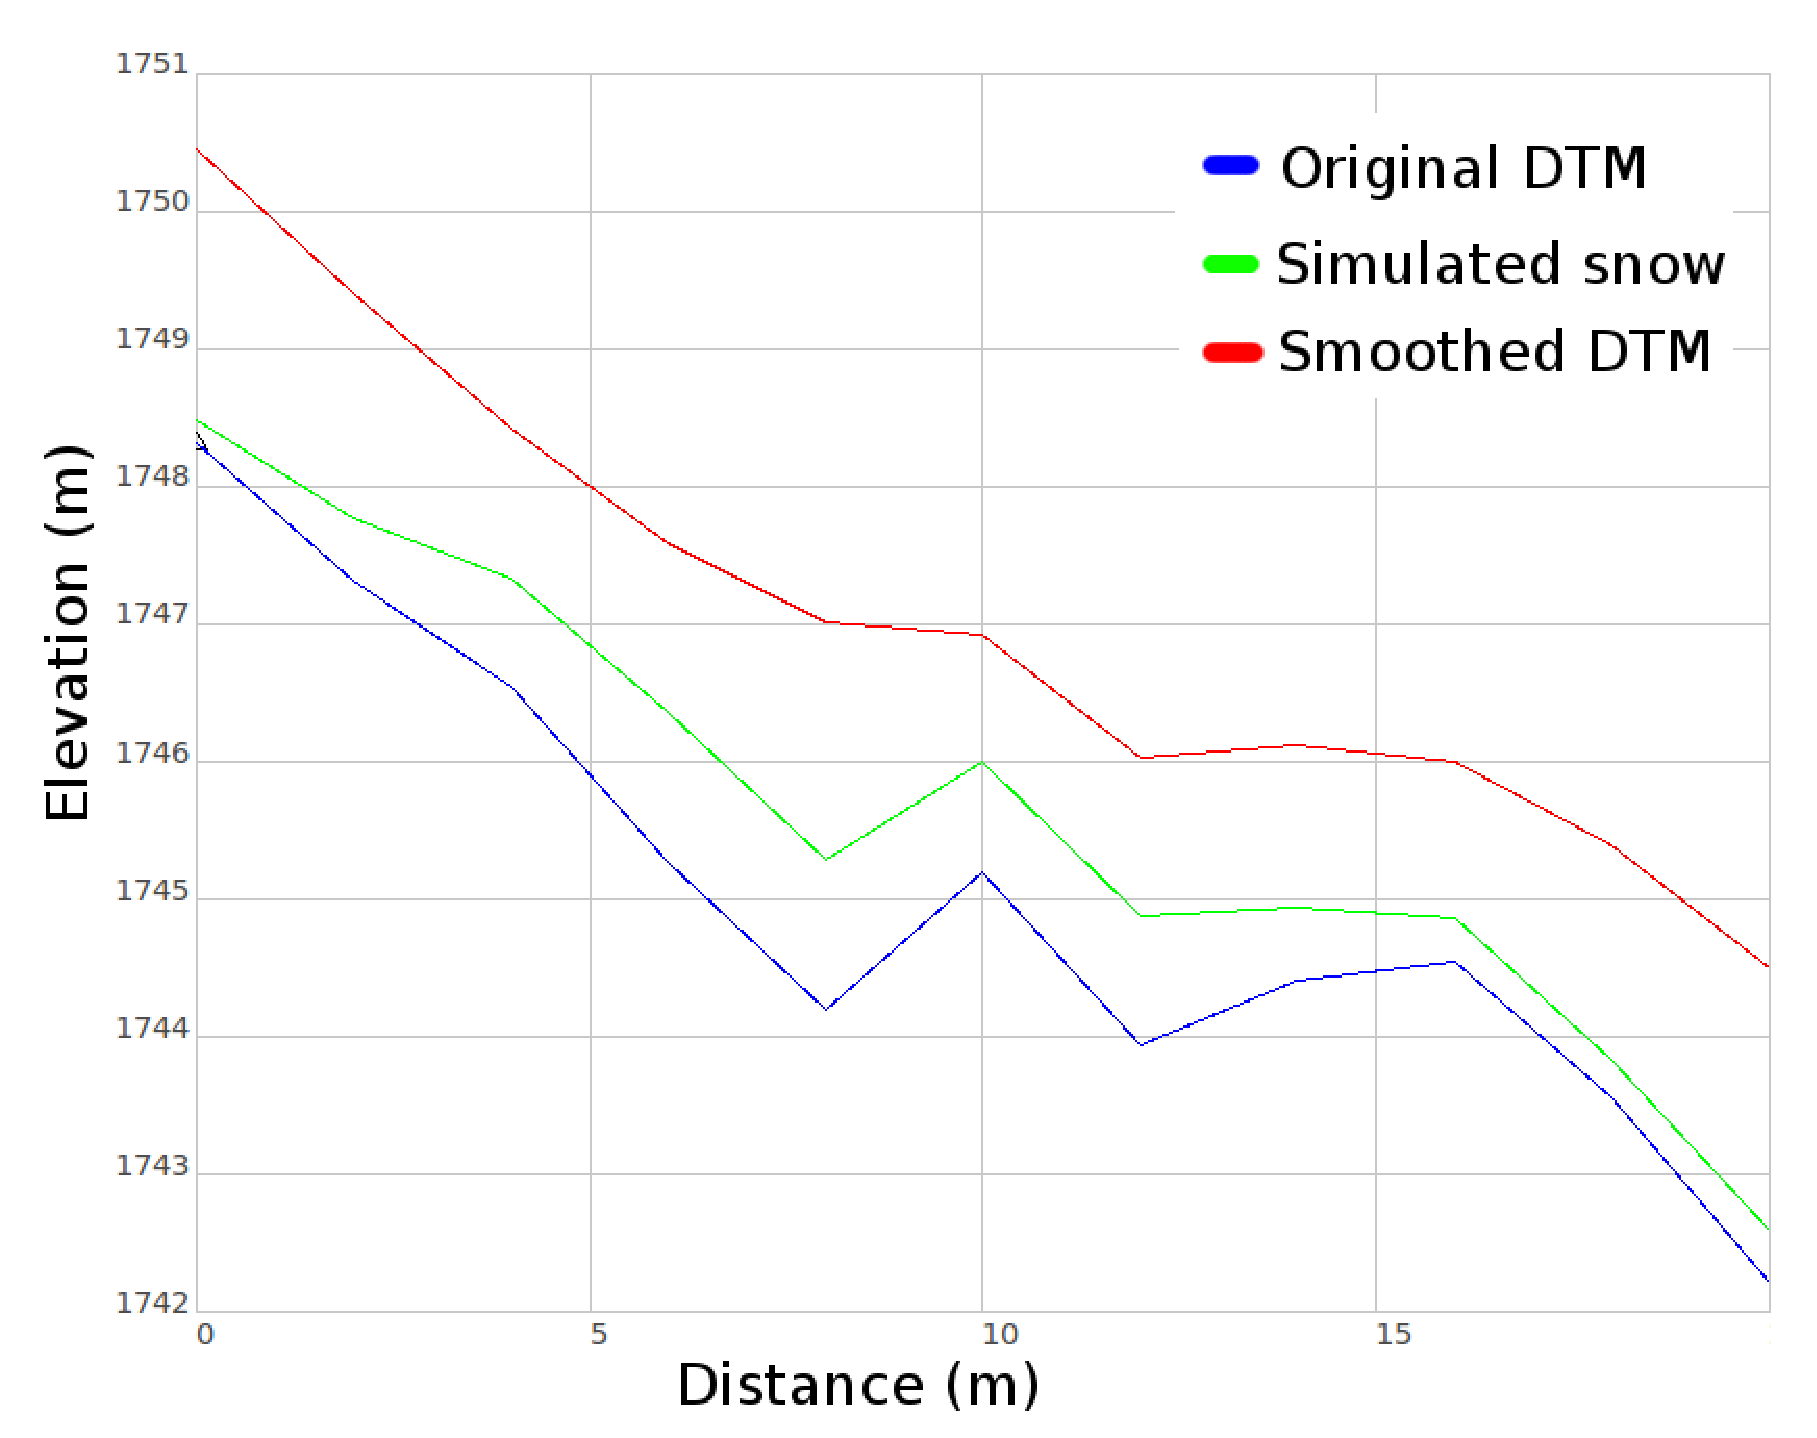
\includegraphics[width=\textwidth]{images/profiles_dtm.eps}
    \caption{Profiles of the dtm and of the simulated dtm after rain fall}\label{profile_dtm}
  \end{center}
\end{figure}

Starting from the smoothed DTM, slope raster map and aspect raster map were computed. The GRASS module r.slope.aspect was used. The slope raster map contains the slope, stated in degree of inclination from the horizontal. The slope of a cell is the maximum rate of change in value from that cell to its neighbors. Conceptually, computing the slope is equivalent to fits a plane to the z-value of a 3x3 neighborhood around the center cell. The slope value of this plane is computed using the average maximum technique(see. \cite{bur2009}). The direction the plan faces is the aspect.

The simulation requires as input the vector map with the polygon of the ski slope for which the model should be run. The ski slope (see. Fig.\ref{uno_tognola_3d} for an example) is extracted from a vector map containing the polygons of slopes of the skiing resort in Trentino. This data are available inside the SicurSkiWeb project and were derived starting from orthophotos and tuned with measurements done in place. From the polygon of the ski slope left and right edge, start and stop areas are derived.

\begin{figure}[!ht]
  \begin{center}
    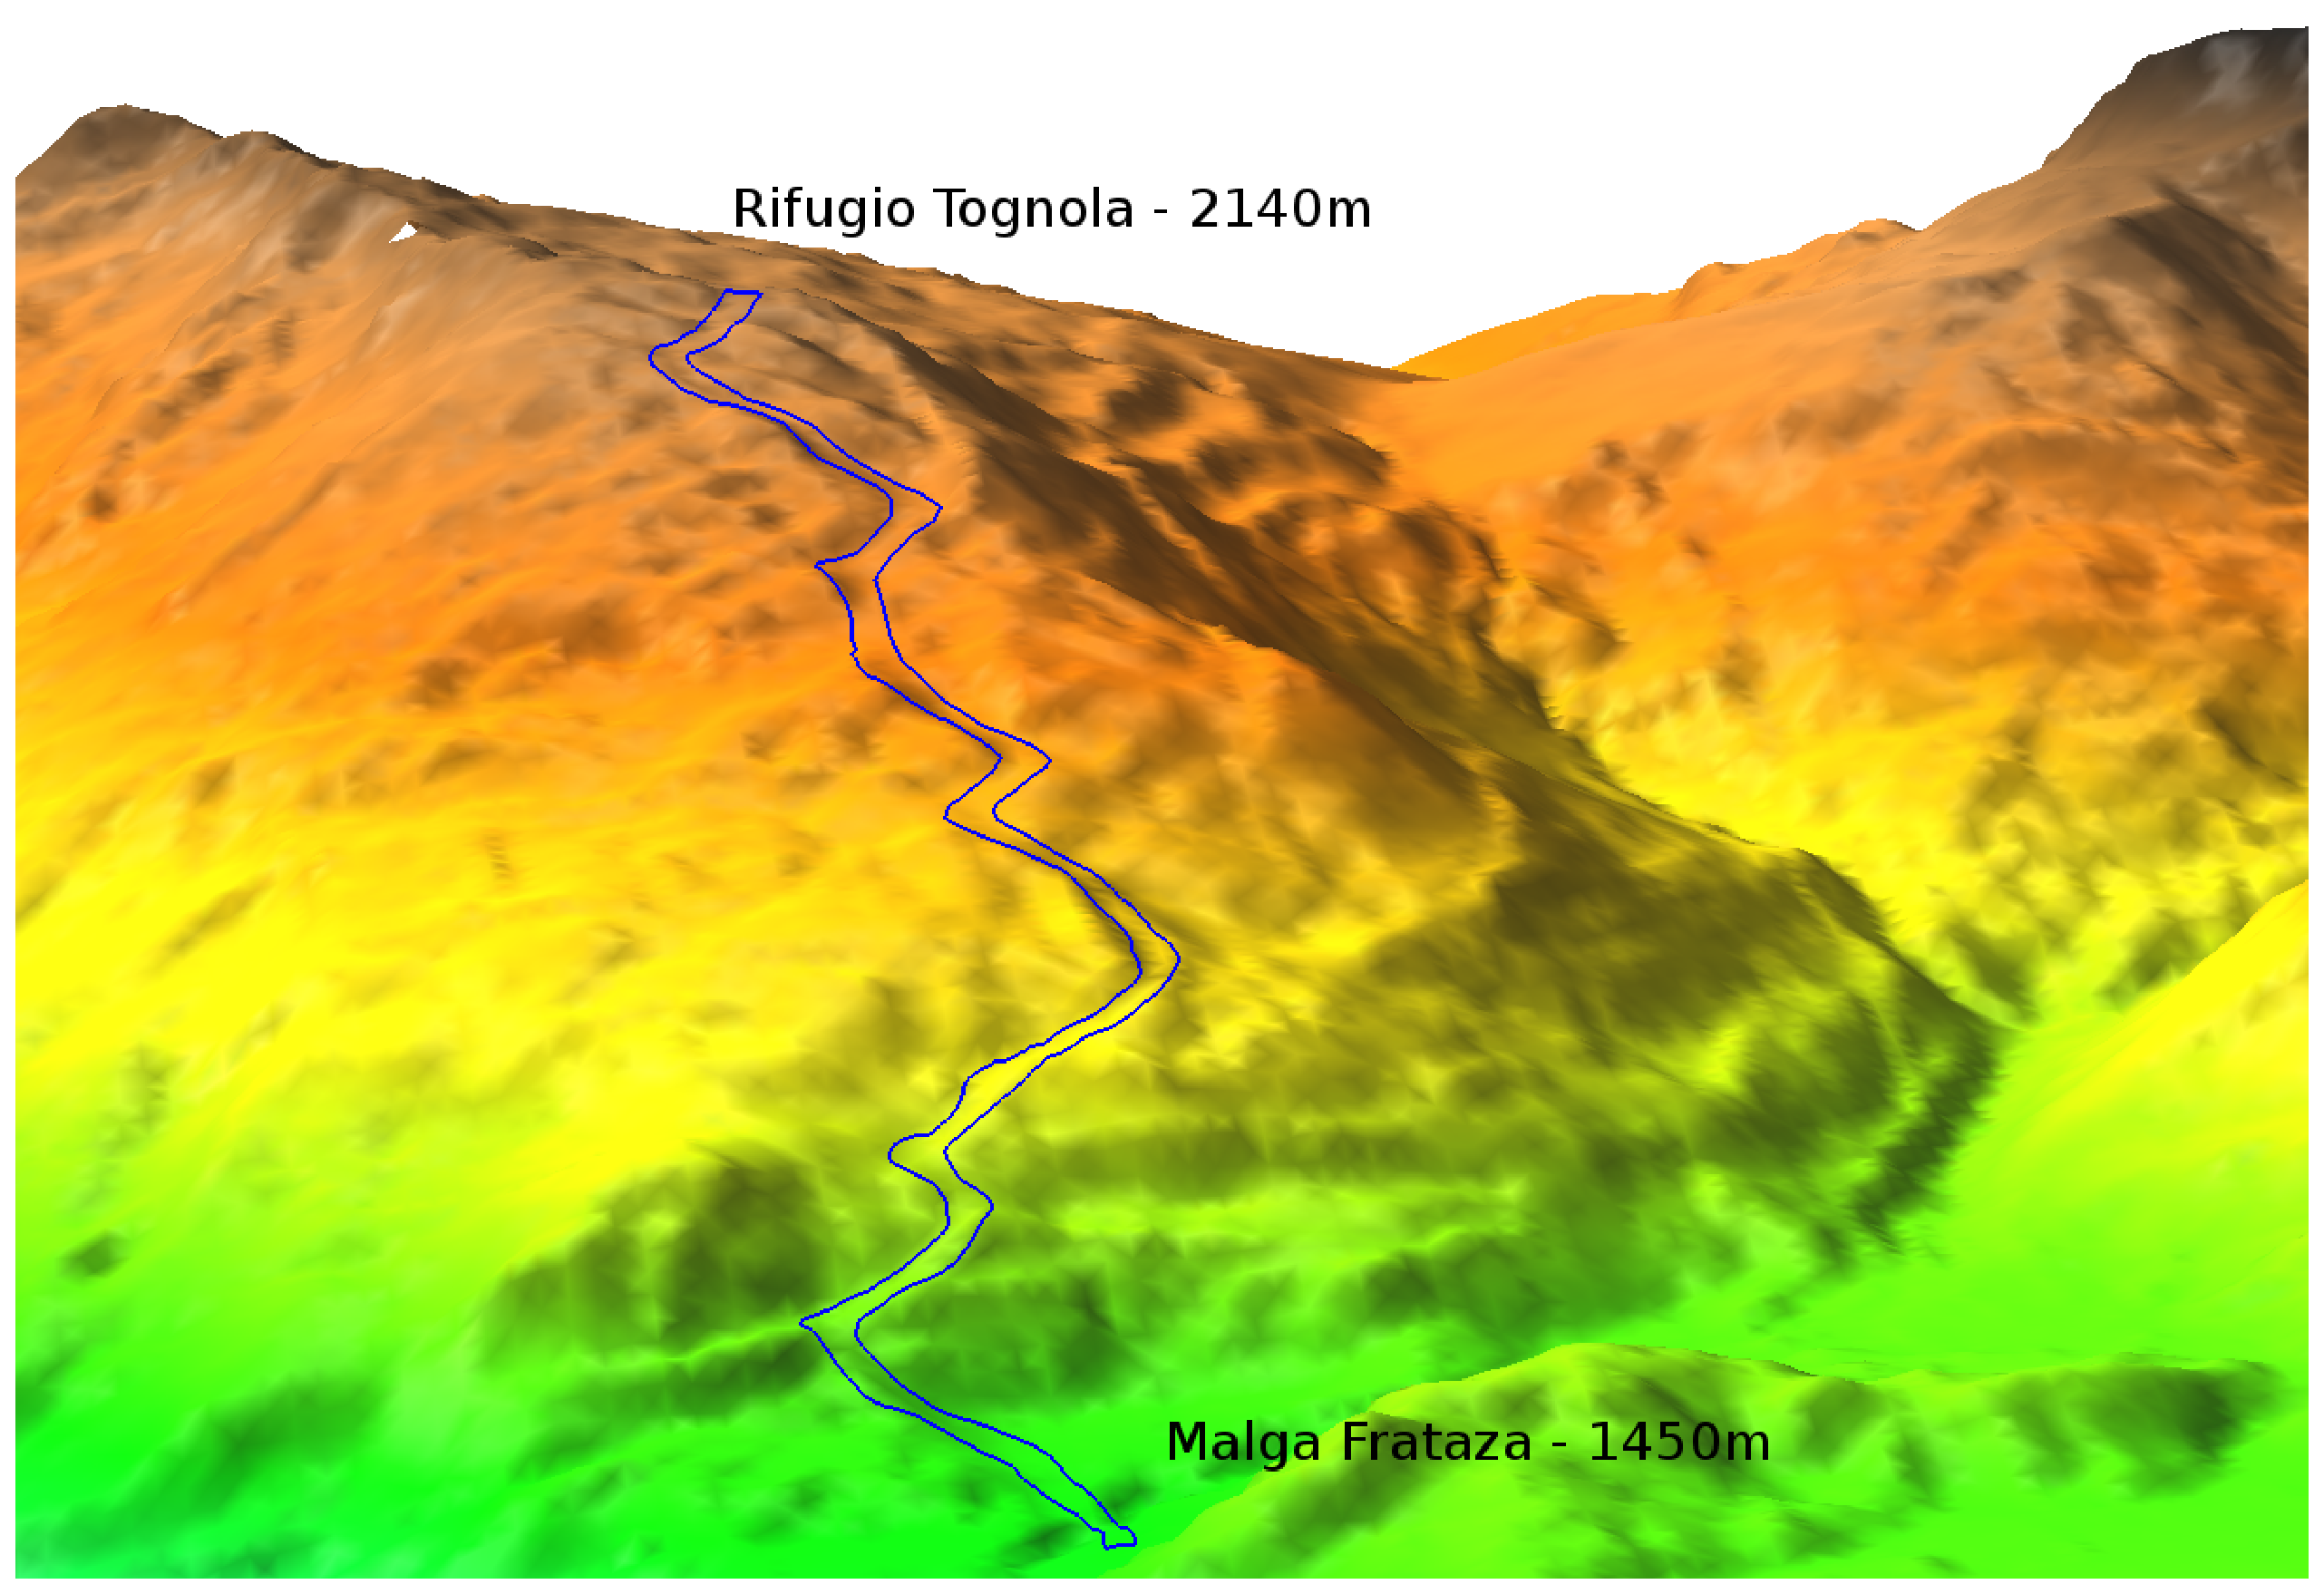
\includegraphics[width=\textwidth]{images/uno_tognola_3d.eps}
    \caption{3d visualization of the ski slope ``Uno di Tognola'' polygon (in blue) in San Martino di Castrozza.}\label{uno_tognola_3d}
  \end{center}
\end{figure}

\section{Output data}\label{output_data}
The output produced by the simulation is the status of each skier at each integration step of the simulation. The information logged at a time $t$ for a skier $a$ are the position $r_a$ and the velocity $\dot{r}_a$.

Starting from this data two main analysis have been performed: speed average and average density of skiers computation. To analyze the speed of skiers along the ski slope a raster map of average speed has been produced. The map is obtained interpolating the speed values simulated by the simulation (see fig.\ref{uno_tognola_speed}). The interpolation was done using the GRASS module v.surf.idw. The GRASS module v.kernel was used to compute the density of skiers on the slope. The raster density map is computed using a moving kernel with gaussian distribution (see fig.\ref{uno_tognola_density}).

\begin{figure}[!ht]
  \begin{center}
    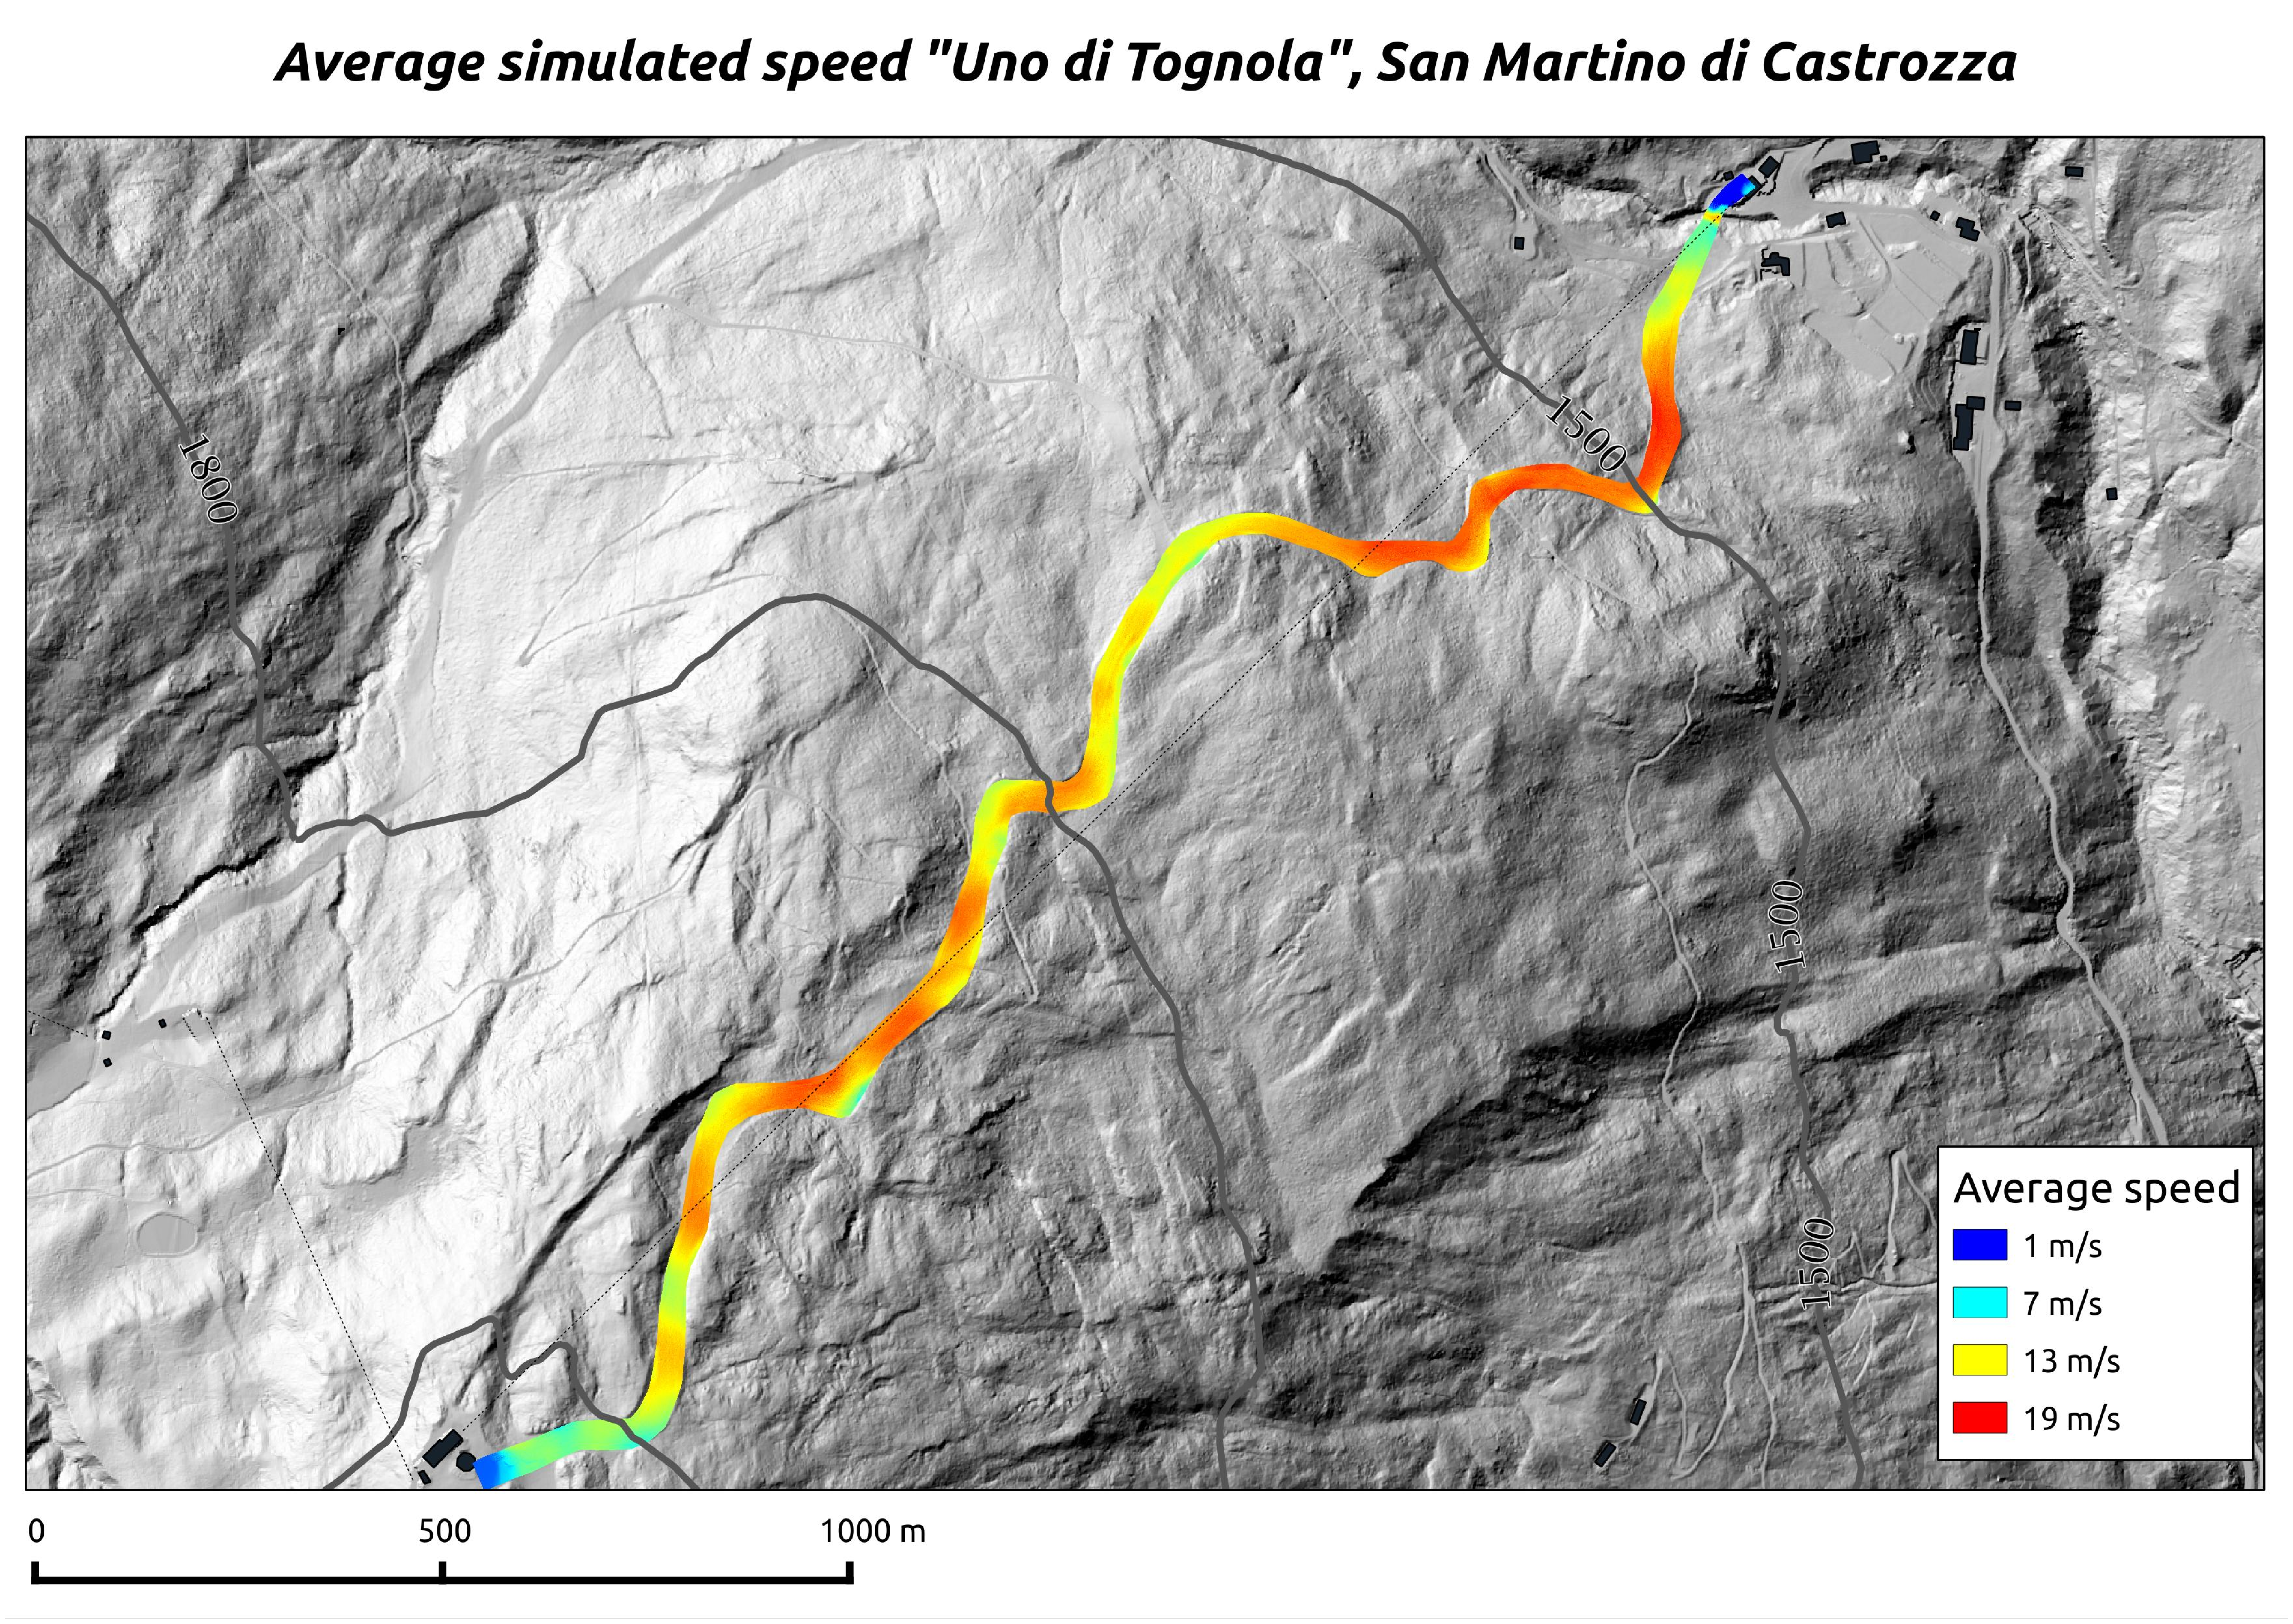
\includegraphics[width=\textwidth]{images/vel_map_sm.eps}
    \caption{Average simulated speed map for the ``Uno di Tognola'' ski slope in San Martino di Castrozza.}\label{uno_tognola_speed}
  \end{center}
\end{figure}

\begin{figure}[!ht]
  \begin{center}
    \includegraphics[width=\textwidth]{images/sm_density_map.eps}
    \caption{Simulated skiers density map for the ``Uno di Tognola'' ski slope in San Martino di Castrozza.}\label{uno_tognola_density}
  \end{center}
\end{figure}

\section{Parameters Selection}
The parameters of the model are of three types: parameters describing the ski slope, parameters regulating the social forces and parameters for the physical forces.

The model assumes that skiers arrive at the beginning of ski slope at a constant rate. Let $\lambda$ be the persons per hour descending a ski slope, then the time between the start of two consecutive skiers is $T=\mathcal{U}\left(\frac{3600}{2/\lambda}\right)$, where $\mathcal{U}(a)$ is the uniform distribution between $0$ and $a$. For the ski slope ``Uno di Tognola'' an arrival rate of $\lambda=200 persons/h$ was chosen.

As in \cite{hol2012} and in \cite{hel2008}, the repulsive potentials defining the social forces are exponential defined as
\begin{align}
U(\norm{r_{aL}})&=U_0 exp(-\norm{r_{aL}}/R_L) \\
U(\norm{r_{aR}})&=U_0 exp(-\norm{r_{aR}}/R_R) \\
V(s)&=V_0 exp(-s/R_A)
\end{align}
where $R_L$, $R_R$ and $R_A$ denote the ranges of the social repulsions, and $U_0$ and $V_0$ are scaling constants that regulate the interaction strength between skiers and the respective object.

The parameters regulating the social forces were set to have forces with equivalent strength and realistic interaction. For the destination force was set $A_0=1$, for the repulsion forces $U_0=10$, $V_0=8$, $R_L=R_R=10$ and $R_A=8$. These choices have the practical implication that the magnitude of the destination force is always equals to $1$ and the repulsion forces tend to $1$ when the skier approximates the edges or other skiers. The angle of view is set to $2\varphi=180°$. As presented in \ref{model}, skiers adjust their direction performing turns when the angle between their direction of motion and the desired direction exceed the angle $\delta$ (see Fig.\ref{start_turn_pic}). This angle was set to $\delta=10°$. The values selected for the social parameters are summarized in table \ref{social_parameters_table}.

\begin{table}
  \begin{center}
  \begin{tabular}{ l | c | c }
    \hline
    Parameter & Symbol & Value \\
    \hline
    Strength of destination force & $A_0$ & 1 \\
    Strength of edge repulsion & $U_0$ & 10 \\
    Strength of athlete repulsion & $V_0$ & 8 \\
    Range of edge repulsion & $R_L=R_R$ & 10 \\
    Range of athlete repulsion & $R_A$ & 8 \\
    Angle of view & $2\varphi$ & 180° \\
    Directional deviation & $\delta$ & 10° \\
    \hline
  \end{tabular}
  \caption{Summary table for parameters regulating social forces}
  \label{social_parameters_table}
  \end{center}
\end{table}

The initialization of the parameters regulating the physical forces was based on values known from the literature. The main reference for choosing the values of the parameters was \cite{hol2012}. The density of air was set to $\rho_{air}=1.3163 kg/m^{-3}$, the mass of the skiers, including clothes and equipment, to $m=85 kg$. The gravitational acceleration was taken equals to $g=9.81 m/s$. The sidecut radius of the skis was set to $R_{SC}=10 m$. According to the values suggested in \cite{bu2004}, the kinetic friction coefficient was set to $\mu = 0.05$. The air drag coefficient $C_d = 1.0$ was chosen and the frontal area was set to $A=0.6 m^2$. These values are summarized in table \ref{physical_parameters_table}.

\begin{table}
  \begin{center}
  \begin{tabular}{ l | c | c }
    \hline
    Parameter & Symbol & Value \\
    \hline
    Air density & $\rho_{air}$ & $1.3163 kg/m^{-3}$ \\
    Skier mass & $m$ & $85 Kg$ \\
    Gravitational acceleration & $g$ & $9.81 m/s^2$ \\
    Sidecut radius & $R_{SC}$ & $10m$ \\
    Kinetic friction coefficient & $\mu$ & $0.05$ \\
    Air drag coefficient & $C_d$ & $1.0$ \\
    Frontal area & $A$ & $0.6 m^2$ \\
    \hline
  \end{tabular}
  \caption{Summary table for parameters regulating physical forces}
  \label{physical_parameters_table}
  \end{center}
\end{table}

\section{Optimization}
An analysis of the performances of the software was performed in order to improve the computation time. The section of the software more critical were those sections accessing the files containing the spatial data. These operations, performed by the GrassBackend, were needed to access the data contained in the GRASS map storage and are very time consuming. To speed up the calls to the GrassBackend a caching mechanism was implemented. For the queries requesting raster map values, once a cell value has been fetched it is cached in memory, so that the next queries will access the data quicker. The implementation of the cache was done using the map class available inside the C++ standard library. The map class is an implementation of an associative containers that was used to efficiently store and retrieve values (the raster map values) using keys (the combination of rows and columns). The speed-up reached thanks to the caching mechanism can be seen in figure \ref{speed-up_cache}.

\begin{figure}[!ht]
  \begin{center}
    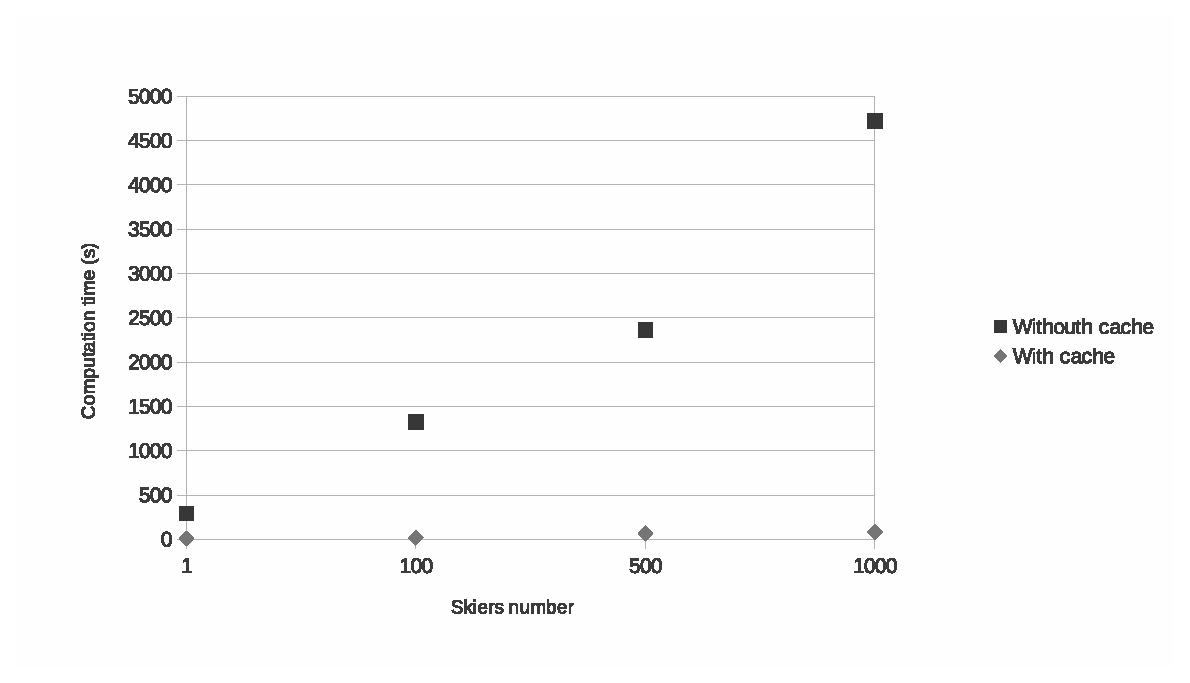
\includegraphics[width=\textwidth]{images/caching.eps}
    \caption{Computation time comparison between simulations with cache and simulation without it}\label{speed-up_cache}
  \end{center}
\end{figure}

\chapter{Steps to validate the model}\label{steps_validate}
\section{Collecting data}
The mobile application SkiLogger was used to collect real data describing the skiers trajectories. SkiLogger is an Android application developed inside the MPBA unit of the Bruno Kessler Foundation. It allows the skiers to track their position using GPS technology while skiing.

SkiLogger was released for beta testing starting from February 2013. At this moment the application does not offer any additional functionality, but for the next seasons it is planned to implement new features such as real time information report about ski slope conditions and traffic, routing trough the ski slope network and friends position tracking. The goal is to incentive more users to use the application and collect a large dataset of real data.

The data collected by the application needs to be filtered: the gps does not always give an accurate position, the application logs every moment including when using the ski lifts. Automated procedures has been developed to individuate and filter the single downhill tracks. As a first elaboration the speed of each point recorded has been computed. In order to minimize the effects of oscillation in the gps measurements, for the recorded position $x_i$ at the time $t_i$, the speed is computed considering the previous and following position as follow
\begin{equation}
v_i=\frac{\norm{x_i-x_{i-1}}+\norm{x_{i+1}-x_i}}{t_{i+1}-t_{i-1}}
\end{equation}

The second step in the processing of data is to filter the track of the skiers on the ski lifts. A sliding window considering sequences of ten points at a time was used. A sequence is valid if the slope between the first and the last point is downhill and greater than a minimum threshold or the skier keeps a minimum value of speed. This is done to exclude sequences tracking movement in flat areas or moving uphill but avoiding to eliminate the sequences tracking movement in area of the ski slope that are counter slope and where skiers should keep a minimum speed to avoid stopping.

Finally, the last step in the cleaning of the data is to isolate the single downhill track. The start of a track is defined as a sequence of at least forty points of the same skier that are within a temporal range and that cover more than a minimum distance. This is useful to eliminate the noise data produced by the gps when skiers stop. In fact, when a skier does not move, if the gps does not have a good precision it tends to jump from different position generating false movement. Once the start of a track is found all the following points, all the following sequences of forty points that are within a time range and that represent a downhill movement are considered to be part of the start track. This last step individuates the single tracks and eliminates the points that are noise related to the inaccuracy of the gps. Figure \ref{data_tognola} shows an example of the data recorded. In some sections of the slope gps inaccuracies can be noted. Sometimes discrepancies can be due also to inaccuracies in the trail of the ski slope.

\begin{figure}[!ht]
  \begin{center}
    \includegraphics[width=\textwidth]{images/data_tognola.eps}
    \caption{Real skiers data logged with the mobile application SkiLogger on the ski slope ``Uno di Tognola'' in San Martino di Castrozza}\label{data_tognola}
  \end{center}
\end{figure}

For the season 2012/2013 a total of 178502 meters of descent has been tracked divided in 115 separate tracks. The average length of the tracks is of 1552 meters. 100 tracks are longer than 500 meters (Table \ref{descendts}).

\begin{table}
  \begin{center}
  \begin{tabular}{ | l | c | }
    \hline
    Total number of tracks & 115 \\ \hline
    Total meters tracked & 178502m \\ \hline
    Average length for track & 1552m \\ \hline
    Tracks longer than 500m & 100 \\
    \hline
  \end{tabular}
  \caption{Summary table for tracks data logged}
  \label{descendts}
  \end{center}
\end{table}

The total number of skiers that has used the application is 18. Each skier was request to fill in a little form before using the application. The data asked included a self-assessment of the skiing skill, the kind of tool used (skis, snowboard, telemark...), the dimension of the group and the age group. Only two skiers chose the beginner level and tracked a 6 tracks for a total of 906 meters. Three skiers were intermediate, with 6 tracks and 6264 meters tracked. Thirteen skiers were experts, they logged 103 tracks and 171331 meters (Table \ref{skiers}).

\begin{table}
  \begin{center}
  \begin{tabular}{ c | c | c | c }
    \hline
    Level & Skiers number & Tracks & Total meters \\
    \hline
    Beginner & 2  & 6 & 906m \\
    Intermediate & 3 & 6 & 6264m \\
    Expert & 13 & 103 & 171331m \\
    \hline
  \end{tabular}
  \caption{Summary table for skiers that have used SkiLogger}
  \label{skiers}
  \end{center}
\end{table}

The main issue of the data collected is that they are not statistically relevant. Of the total 115 tracks, 52 were tracked by one skier. Another problem is that they are spread on ten different skiing resort in Trentino. For this reason we have very few ski slopes that were tracked by different skiers. In particular there are only two slopes with 5 or 4 different skiers, 8 slopes with 3 skiers and 62 slopes with 1 or 2 skiers (Table \ref{slopes}).

\begin{table}
  \begin{center}
  \begin{tabular}{ c | c }
    \hline
    Different skiers & Slopes number \\
    \hline
    5 & 1 \\
    4 & 1 \\
    3 & 8 \\
    2 & 18 \\
    1 & 44 \\
    \hline
  \end{tabular}
  \caption{Table summarizing the number of different skiers for the ski slopes}
  \label{slopes}
  \end{center}
\end{table}

The data collected does not allow to do a realistic tuning of the parameters and to validate the model for ski slopes in Trentino. However some comparisons between the data collected and the simulated data has been performed.

\section{Simulated vs. real data}
The data collected are to few to analyze the map of skiers density produced. Instead, this part of the analysis focuses on the difference between the speed estimated by the simulation and the speed recorded by the SkiLogger application. Starting from the map of simulated speed (see Figure\ref{uno_tognola_speed}), produced as described in section \ref{output_data}, the values of speed computed for each point tracked by the application was compared to the values of speed of the map. Figure \ref{sm_track47} shows the comparison between real and simulated values of speed for the track 47 of the skier 15 recorded on the ski slope ``Uno di Tognola'': while the simulated skiers do not stop during the descent the skier stopped at least three times.

\begin{figure}[!ht]
  \begin{center}
    \includegraphics[width=\textwidth]{images/sm_track47.eps}
    \caption{Comparison between simulated and real speed for the track 47 on the ski slope ``Uno di Tognola''}\label{sm_track47}
  \end{center}
\end{figure}

For each track recorded on the ski slope were computed the error between real and simulated values as $e=v_R-v_S$ where $v_R$ is the real speed recorded and $v_S$ the speed simulated by the model. Figure \ref{map_error} show the map of the error made for each point of the tracks. The point in the map were the skiers error is higher is were the skiers stopped. It can be seen that the error produced by the stops reverberates on the following points. To compare the speed values taking into account the stops a new simulation was run where the simulated skiers were forced to stop according to the stops made by the skier 35 in the track 116. A new map of simulated speed were interpolated, Figure \ref{sm_stops_track116} shows the comparison for the track 116.

\begin{figure}[!ht]
  \begin{center}
    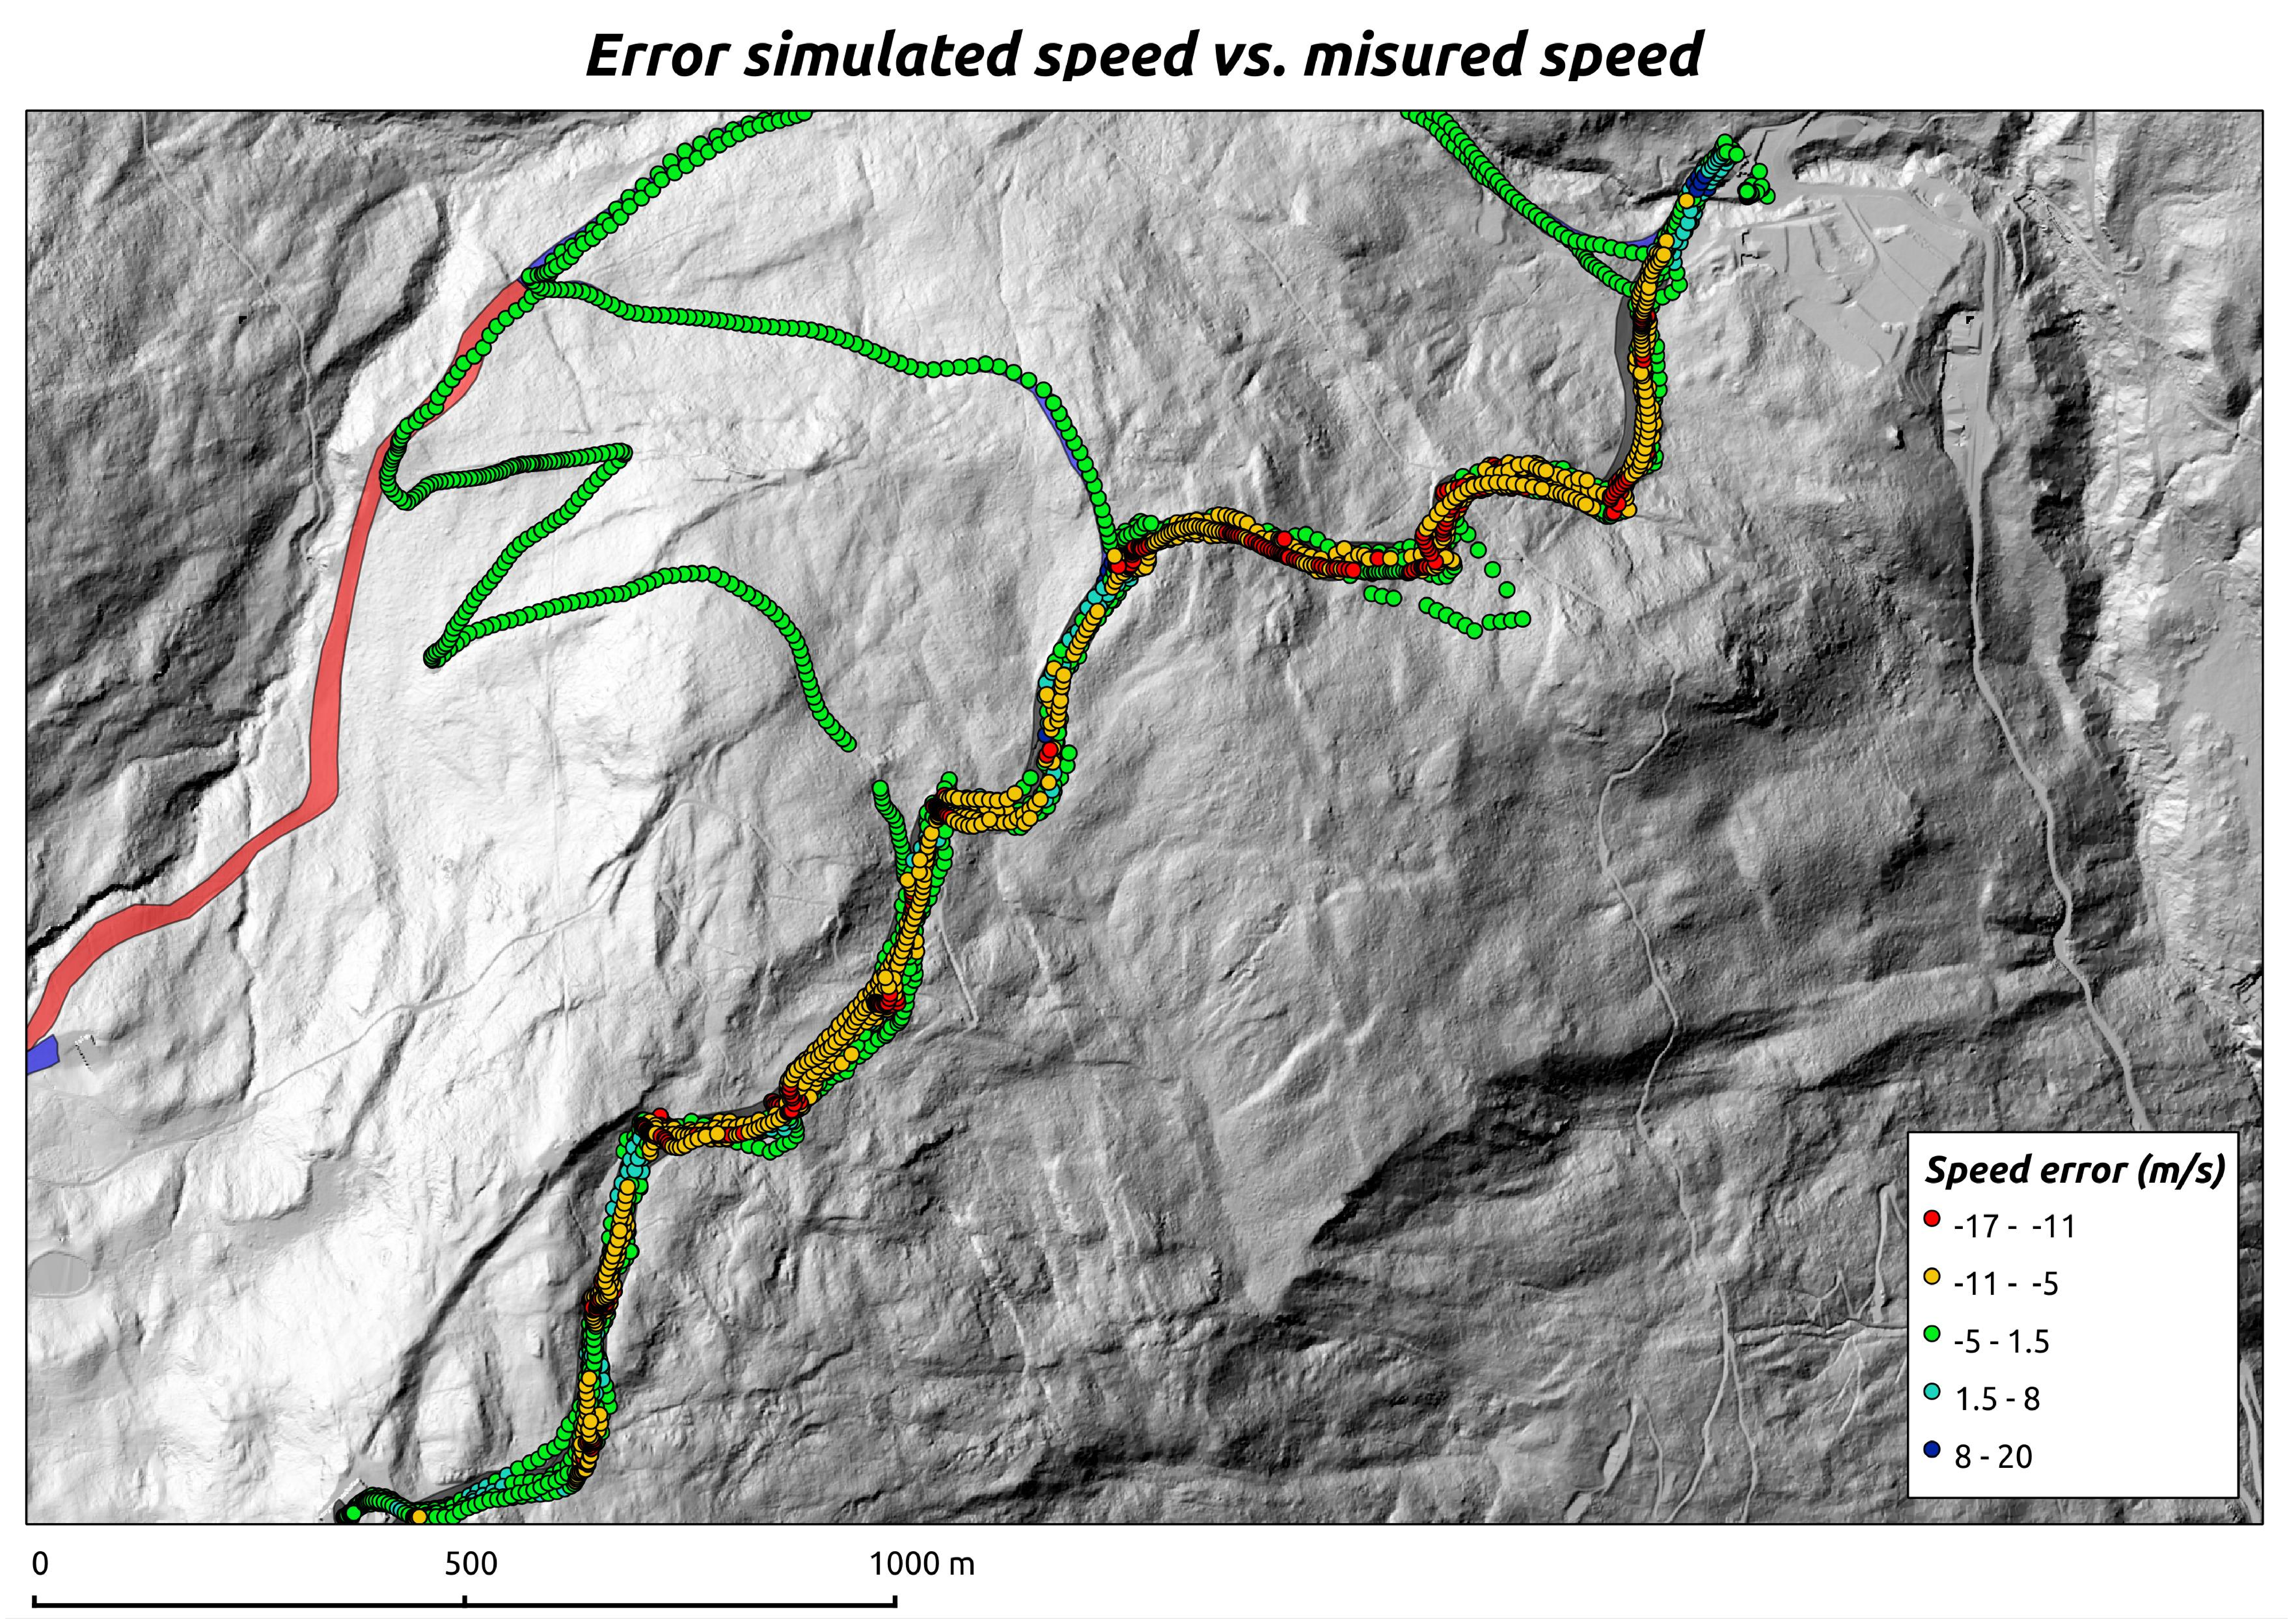
\includegraphics[width=\textwidth]{images/map_error.eps}
    \caption{Map of the errors between the real and the simulated speed on the tracks recorded on the ski slope ``Uno di Tognola''}\label{map_error}
  \end{center}
\end{figure}

\begin{figure}
        \centering
        \begin{subfigure}[b]{0.5\textwidth}
                \centering
                \includegraphics[width=\textwidth]{images/sm_track116.eps}
                \caption{}
                \label{Sno_stops}
        \end{subfigure}%
        ~ %add desired spacing between images, e. g. ~, \quad, \qquad etc.
          %(or a blank line to force the subfigure onto a new line)
        \begin{subfigure}[b]{0.5\textwidth}
                \centering
                \includegraphics[width=\textwidth]{images/sm_stops_track116.eps}
                \caption{}
                \label{Sstops}
        \end{subfigure}
        \caption{Simulated and real speed values for track 116 of ``Uno di Tognola''. Figure \ref{Sno_stops} is without stops, in Figure \ref{Sstops} simulated skiers were forced to stop as the real skier}\label{sm_stops_track116}
\end{figure}

\chapter{Conclusions}


\bibliography{thesis}
\end{document}